\documentclass{article}\usepackage[]{graphicx}\usepackage[]{xcolor}
% maxwidth is the original width if it is less than linewidth
% otherwise use linewidth (to make sure the graphics do not exceed the margin)
\makeatletter
\def\maxwidth{ %
  \ifdim\Gin@nat@width>\linewidth
    \linewidth
  \else
    \Gin@nat@width
  \fi
}
\makeatother

\definecolor{fgcolor}{rgb}{0.345, 0.345, 0.345}
\newcommand{\hlnum}[1]{\textcolor[rgb]{0.686,0.059,0.569}{#1}}%
\newcommand{\hlstr}[1]{\textcolor[rgb]{0.192,0.494,0.8}{#1}}%
\newcommand{\hlcom}[1]{\textcolor[rgb]{0.678,0.584,0.686}{\textit{#1}}}%
\newcommand{\hlopt}[1]{\textcolor[rgb]{0,0,0}{#1}}%
\newcommand{\hlstd}[1]{\textcolor[rgb]{0.345,0.345,0.345}{#1}}%
\newcommand{\hlkwa}[1]{\textcolor[rgb]{0.161,0.373,0.58}{\textbf{#1}}}%
\newcommand{\hlkwb}[1]{\textcolor[rgb]{0.69,0.353,0.396}{#1}}%
\newcommand{\hlkwc}[1]{\textcolor[rgb]{0.333,0.667,0.333}{#1}}%
\newcommand{\hlkwd}[1]{\textcolor[rgb]{0.737,0.353,0.396}{\textbf{#1}}}%
\let\hlipl\hlkwb

\usepackage{framed}
\makeatletter
\newenvironment{kframe}{%
 \def\at@end@of@kframe{}%
 \ifinner\ifhmode%
  \def\at@end@of@kframe{\end{minipage}}%
  \begin{minipage}{\columnwidth}%
 \fi\fi%
 \def\FrameCommand##1{\hskip\@totalleftmargin \hskip-\fboxsep
 \colorbox{shadecolor}{##1}\hskip-\fboxsep
     % There is no \\@totalrightmargin, so:
     \hskip-\linewidth \hskip-\@totalleftmargin \hskip\columnwidth}%
 \MakeFramed {\advance\hsize-\width
   \@totalleftmargin\z@ \linewidth\hsize
   \@setminipage}}%
 {\par\unskip\endMakeFramed%
 \at@end@of@kframe}
\makeatother

\definecolor{shadecolor}{rgb}{.97, .97, .97}
\definecolor{messagecolor}{rgb}{0, 0, 0}
\definecolor{warningcolor}{rgb}{1, 0, 1}
\definecolor{errorcolor}{rgb}{1, 0, 0}
\newenvironment{knitrout}{}{} % an empty environment to be redefined in TeX

\usepackage{alltt}
\usepackage[utf8]{inputenc}
\usepackage[parfill]{parskip}
\usepackage[margin=0.75in]{geometry}
\pagenumbering{gobble}
\usepackage{amsmath}
\usepackage{amssymb}
\usepackage[shortlabels]{enumitem}
\usepackage{listings}
\usepackage{graphicx}
\usepackage{subfigure}


\title{Statistics Data Project: Eviction Notices in SF}

\author{Brian Liu}
\date{21 May 2023}
\IfFileExists{upquote.sty}{\usepackage{upquote}}{}
\begin{document}


\maketitle

\section{Introduction}
One of the biggest problems that is beginning to plague America is affordable housing, and San Francisco is a notable city with significant history about the struggle between tenants and landlords with housing. It not only has a known problem with unaffordable housing from the tech booms bringing significant wage gaps, but it also has a rich amount of data telling the stories for hundreds of thousands tenants that have been evicted from their homes. In this paper, I will explore the eviction notices published by SF Rent Board in San Francisco. I will look at the different types of evictions, the neighborhoods that are most affected, and the time periods that have the most evictions. I will also look at the different types of evictions and how they change over time.

\subsection{Data}
The data is made up of roughly 222,000 eviction notices from 1997 to 2023. The most important variables that I analyzed are the eviction filing date (FD), longitude (LG), latitude (LT), and eviction type (ET), which includes 18 different types of evictions. I will introduce ETs as they come in this paper.

\section{Exploratory Data Analysis}
\subsection{Mapping Evictions}
\begin{figure}[htbp]
    \centering
    \subfigure[Notices in 1997]{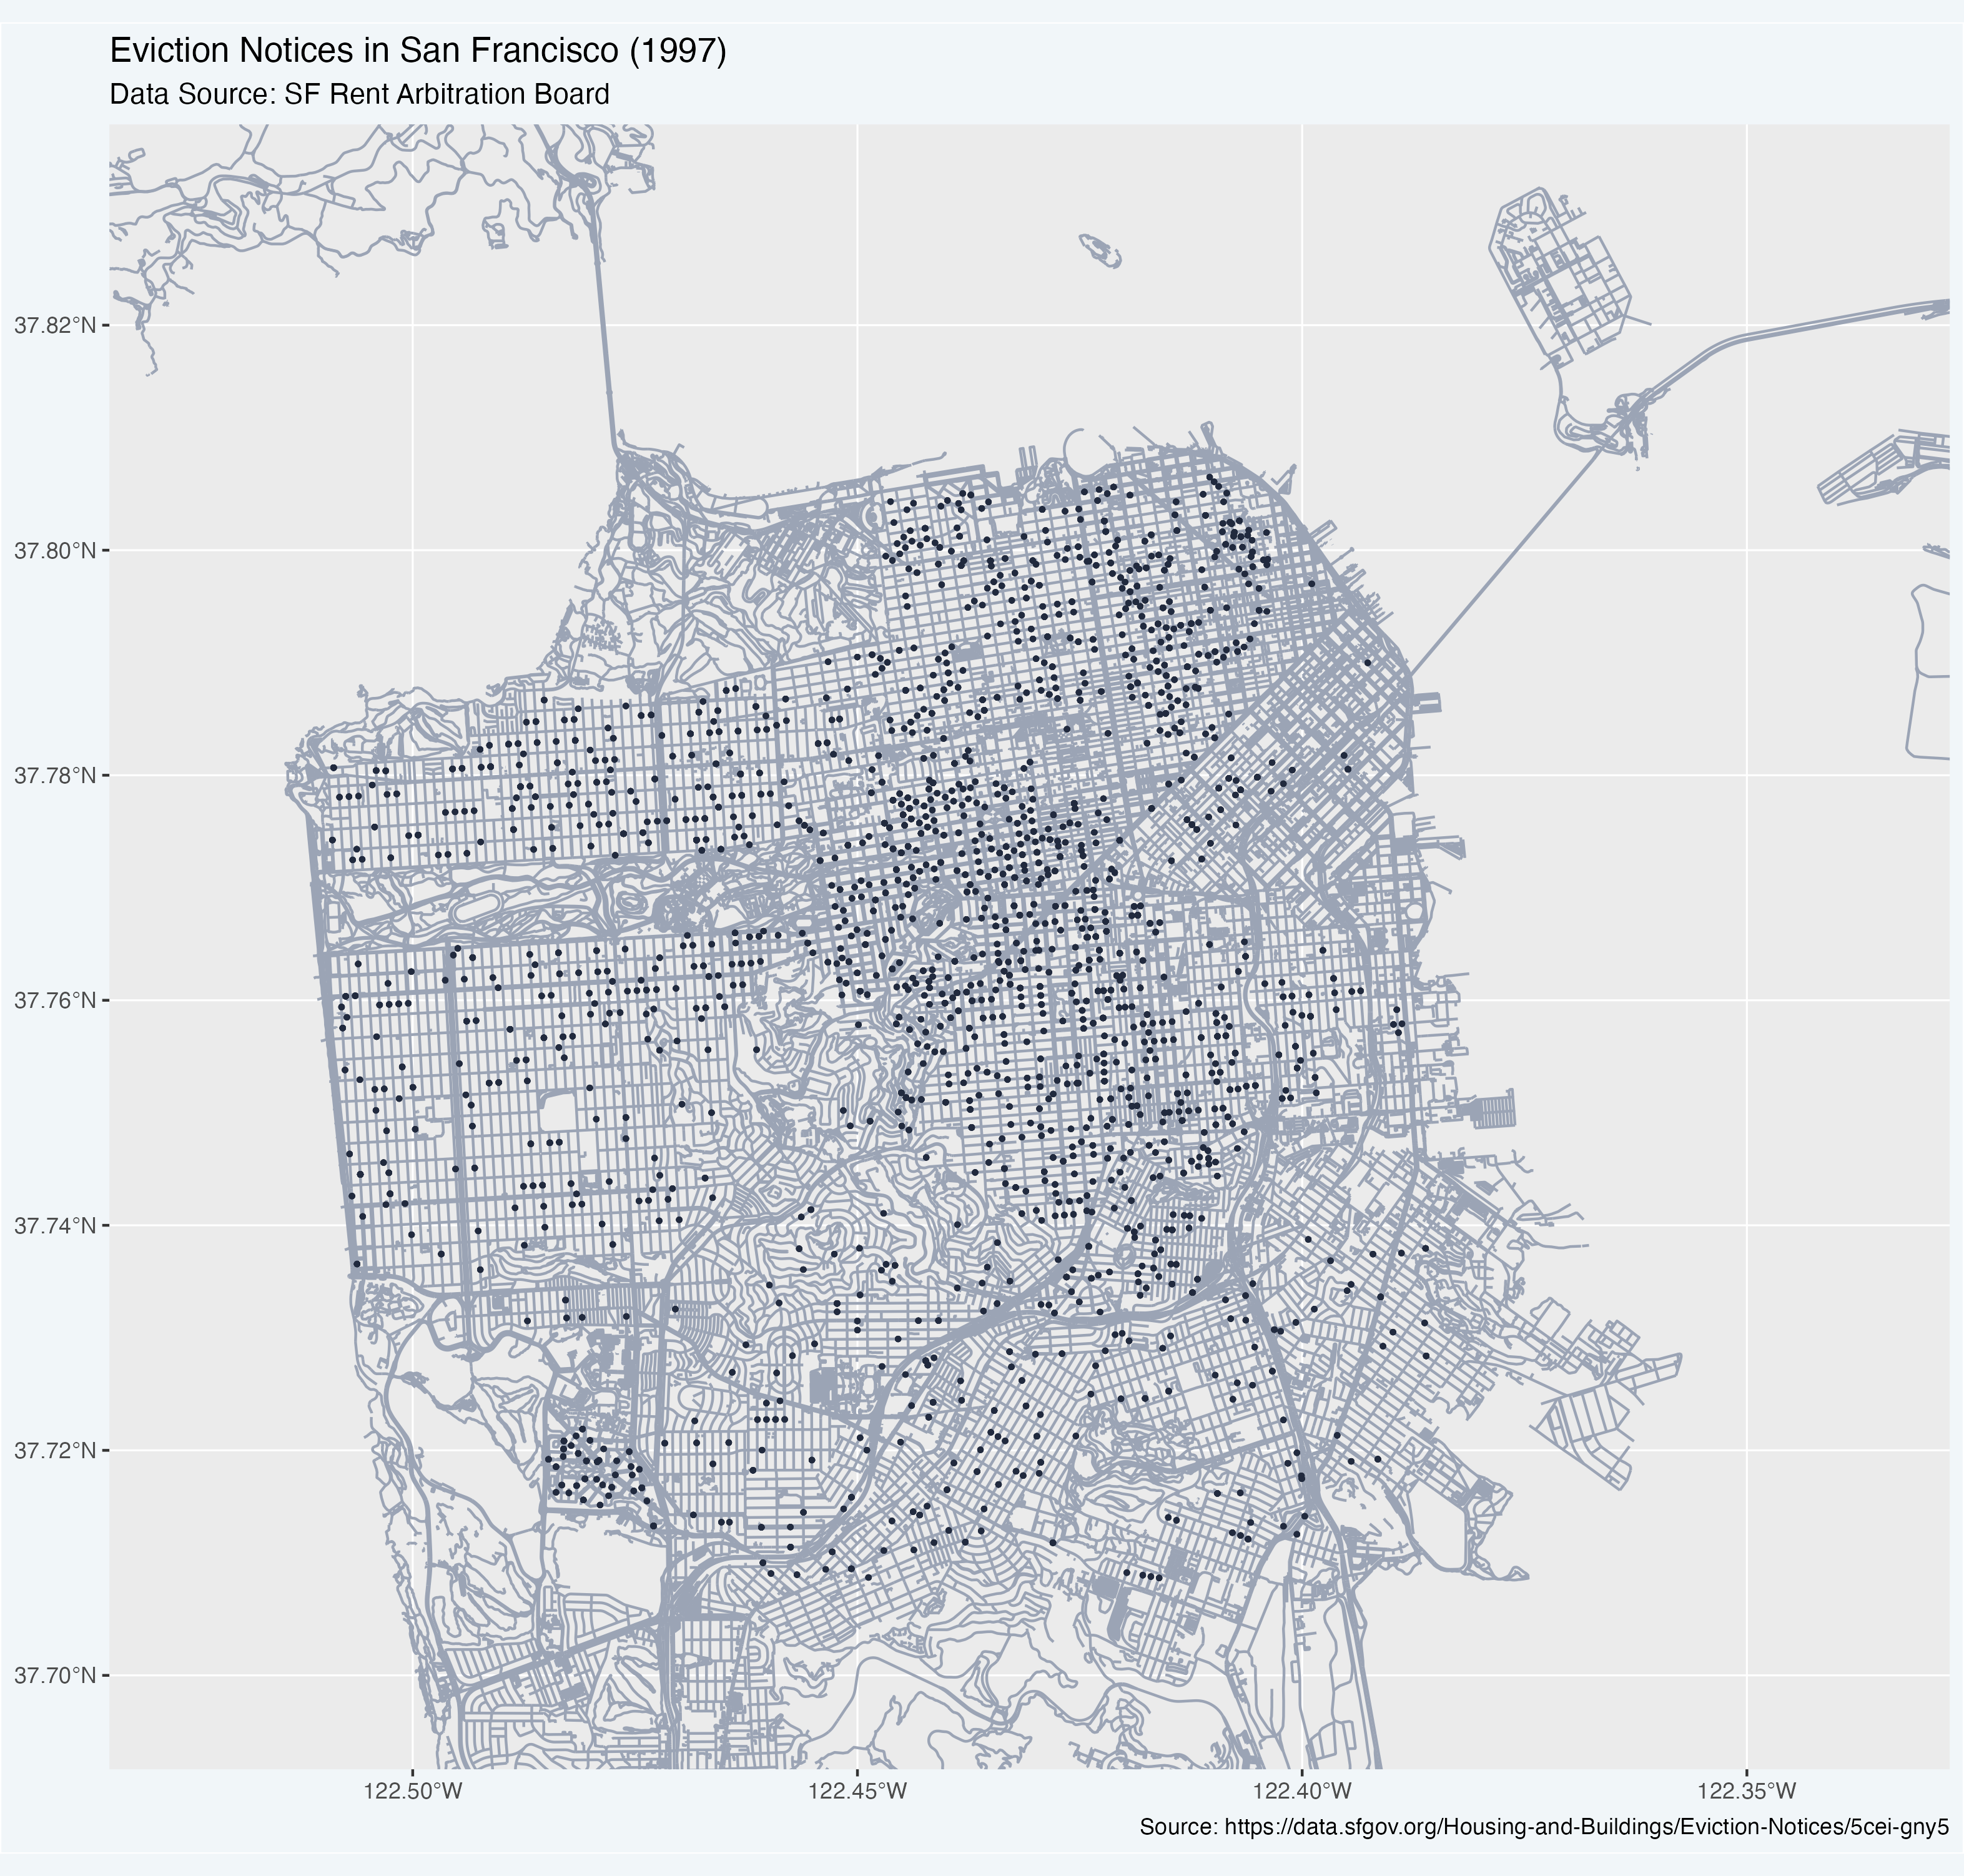
\includegraphics[width=0.3\textwidth]{images/eviction_notices_by_year/1997.png}}
    \subfigure[Notices in 1998]{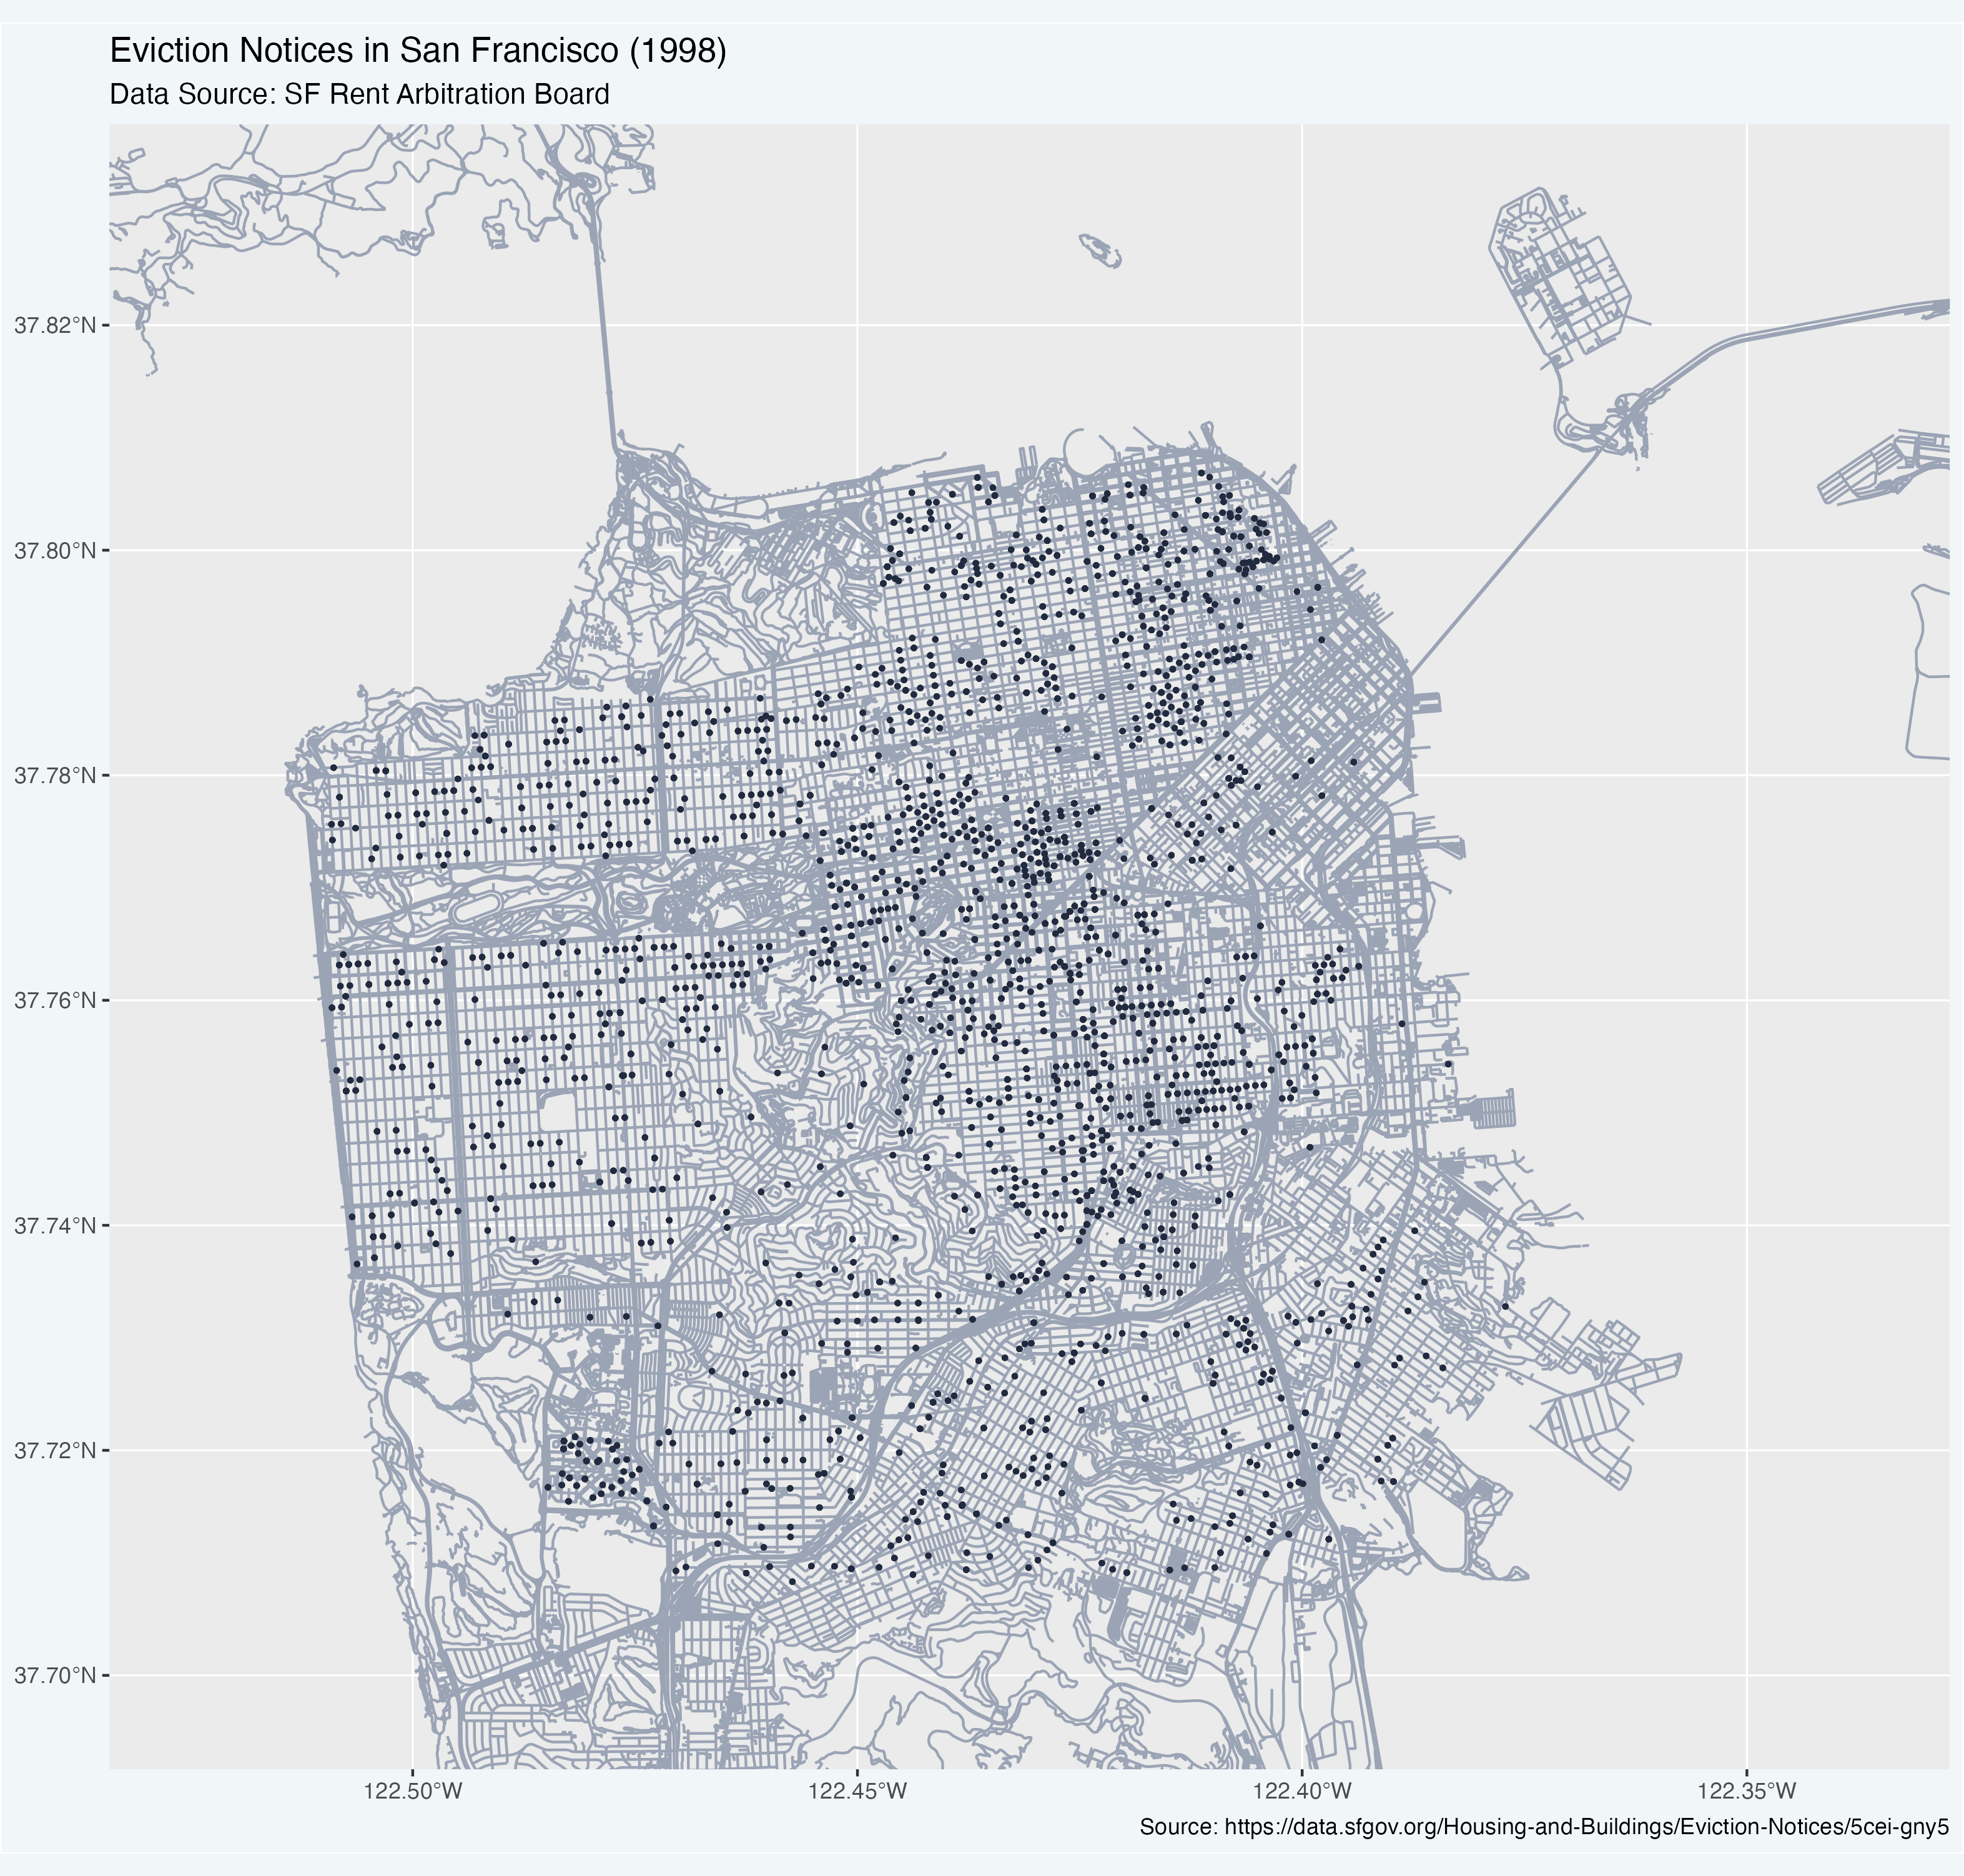
\includegraphics[width=0.3\textwidth]{images/eviction_notices_by_year/1998.png}}
    \subfigure[Notices in 1999]{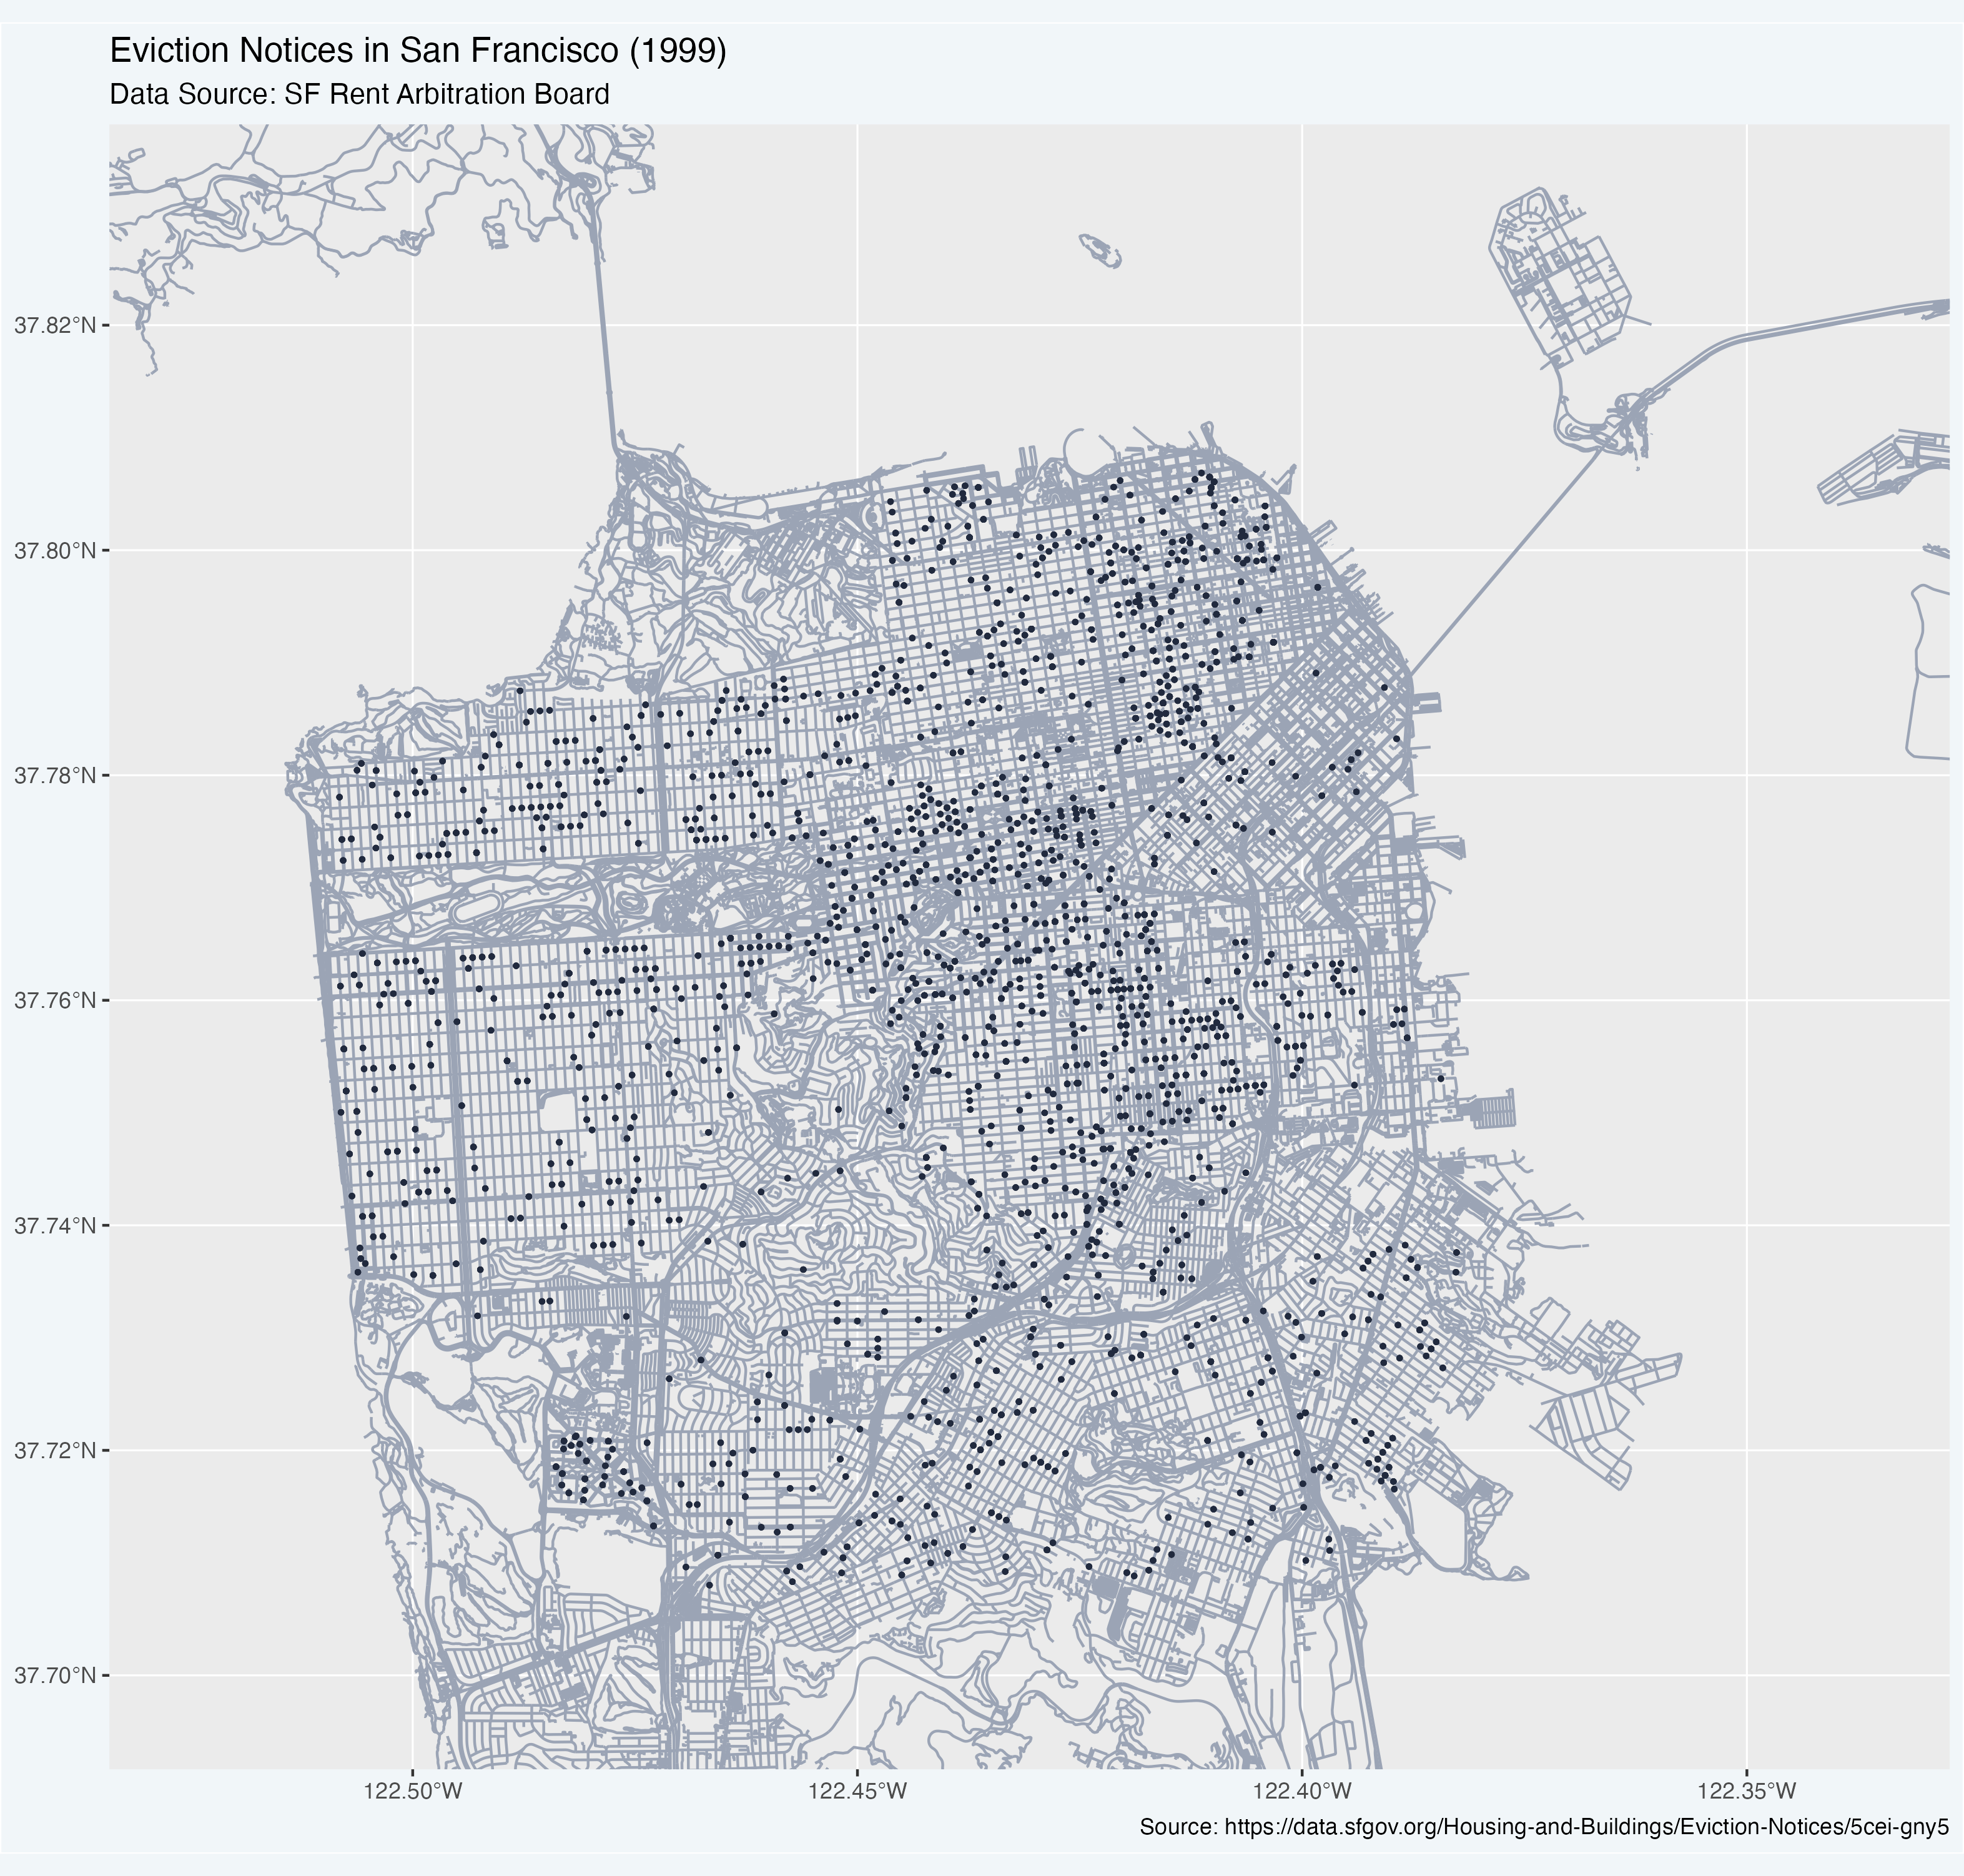
\includegraphics[width=0.3\textwidth]{images/eviction_notices_by_year/1999.png}}
    \subfigure[Notices in 2000]{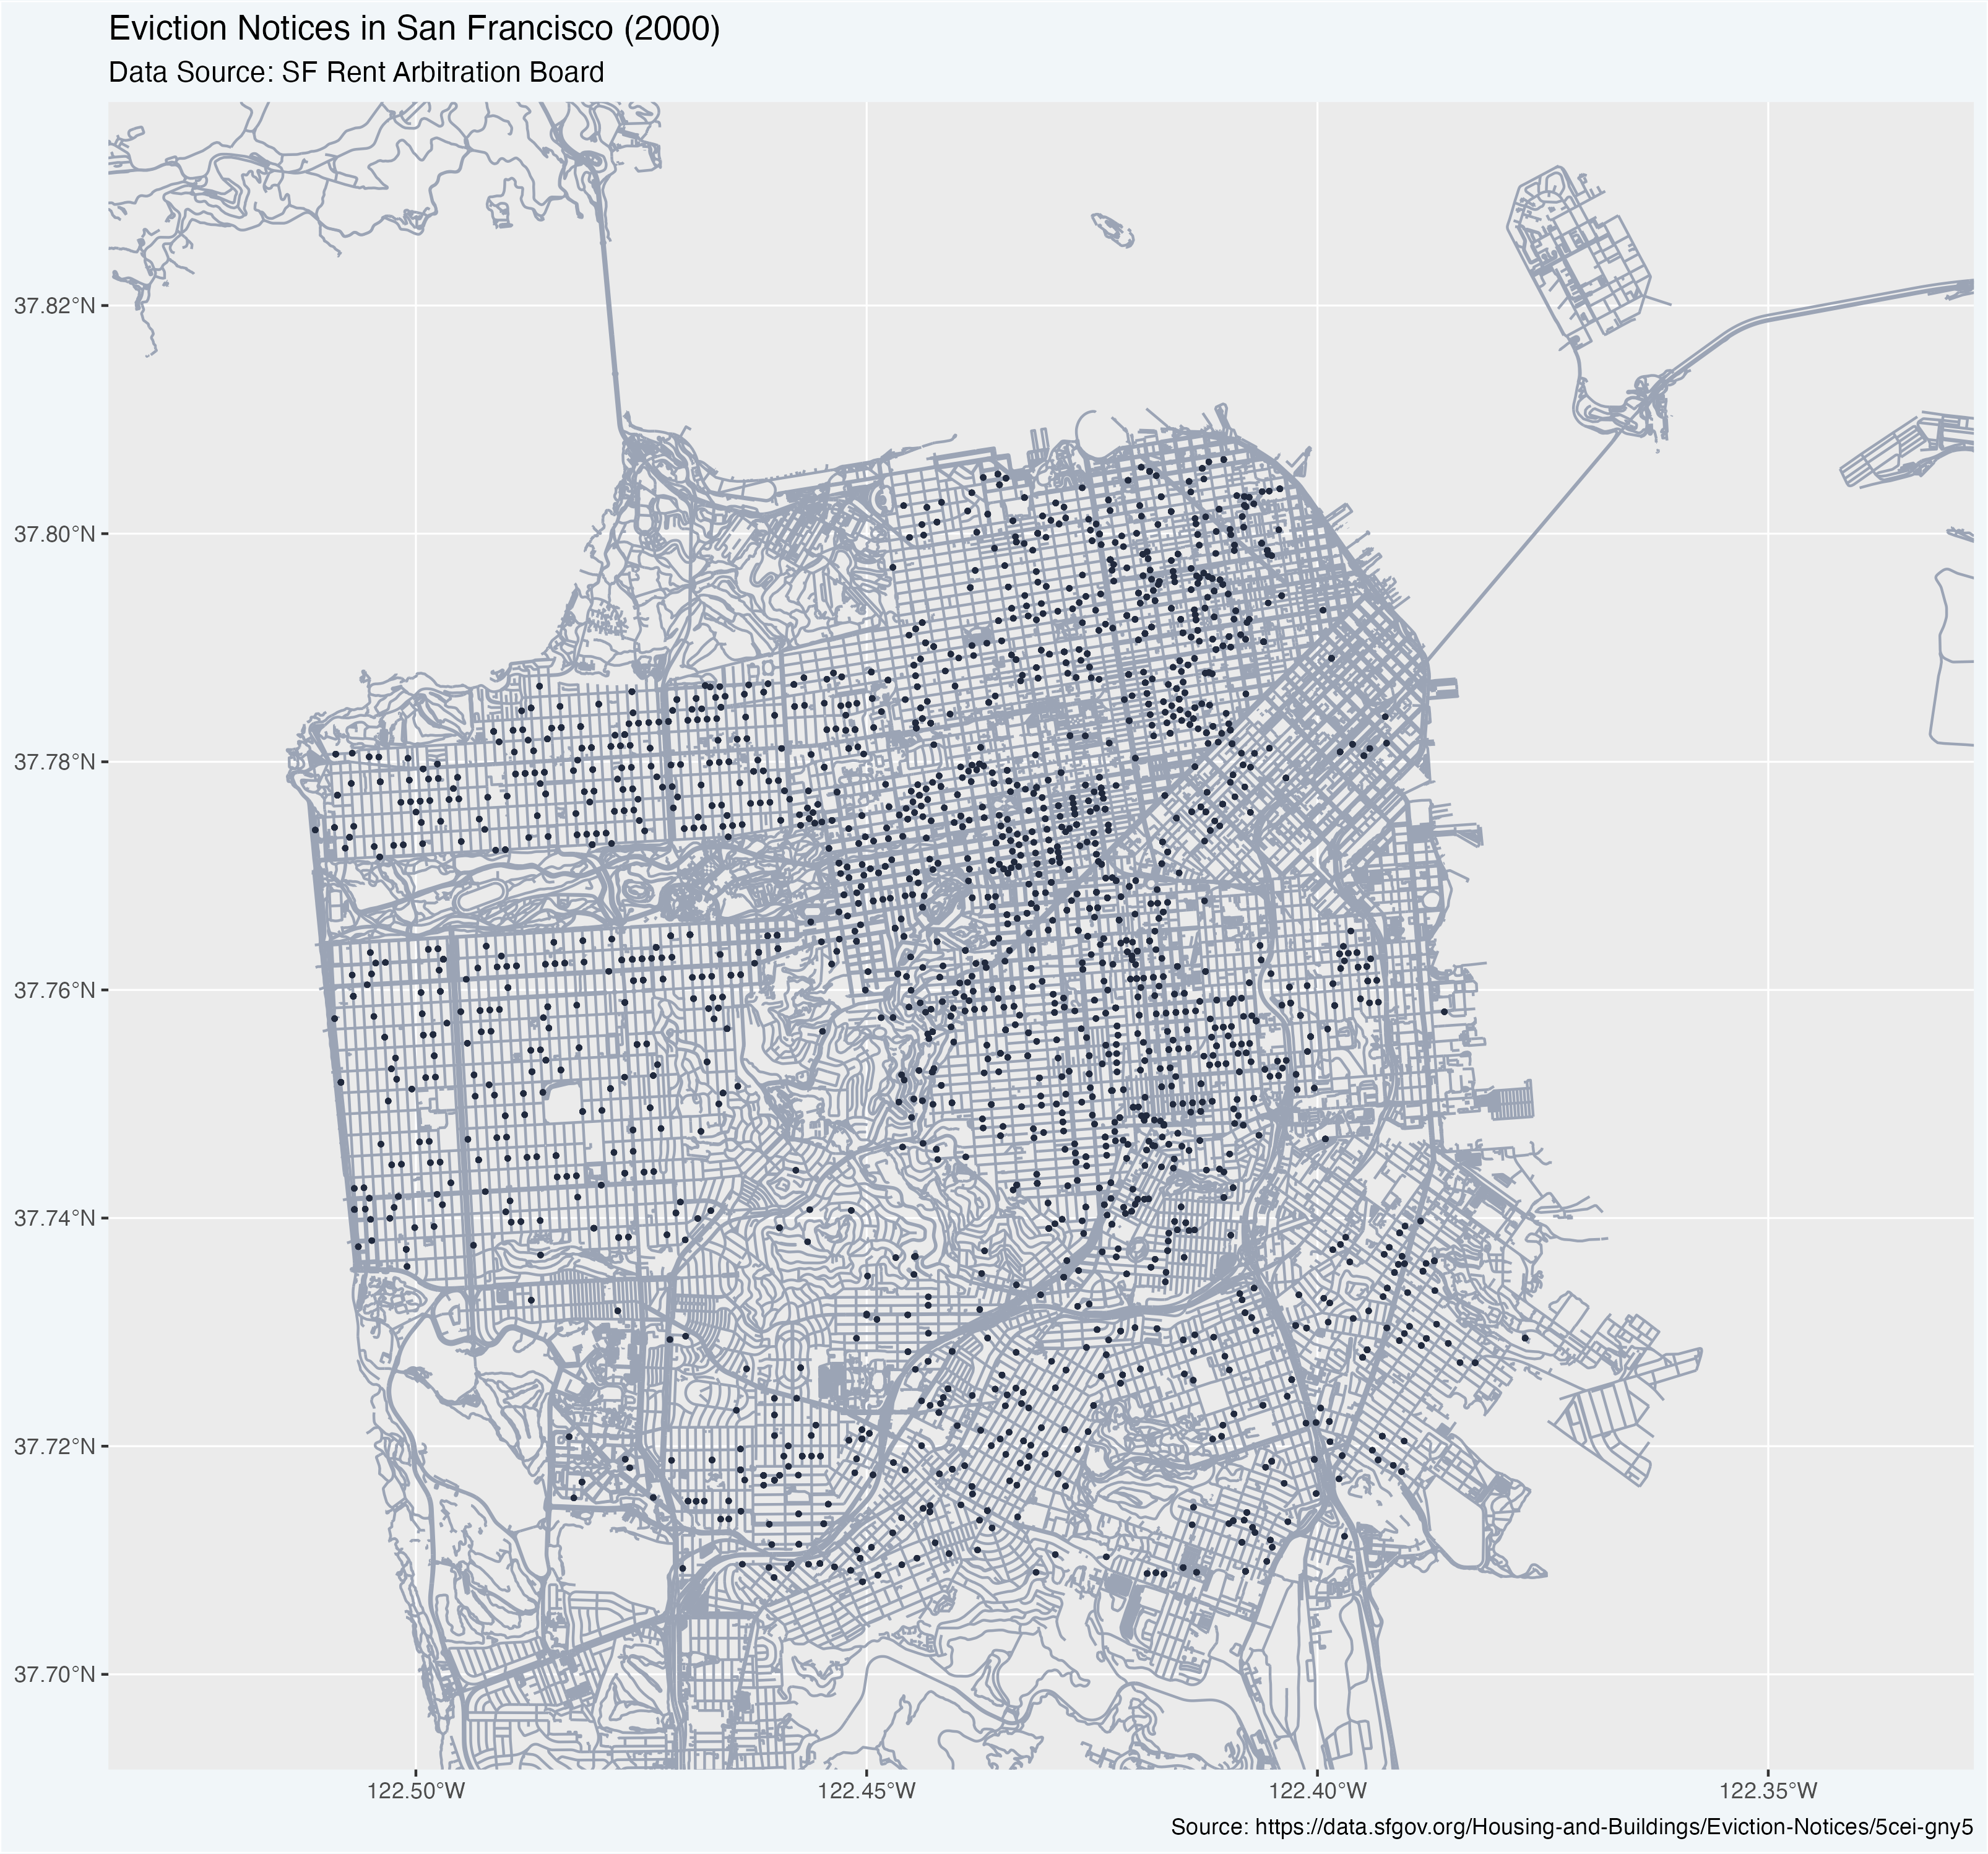
\includegraphics[width=0.3\textwidth]{images/eviction_notices_by_year/2000.png}}
    \subfigure[Notices in 2001]{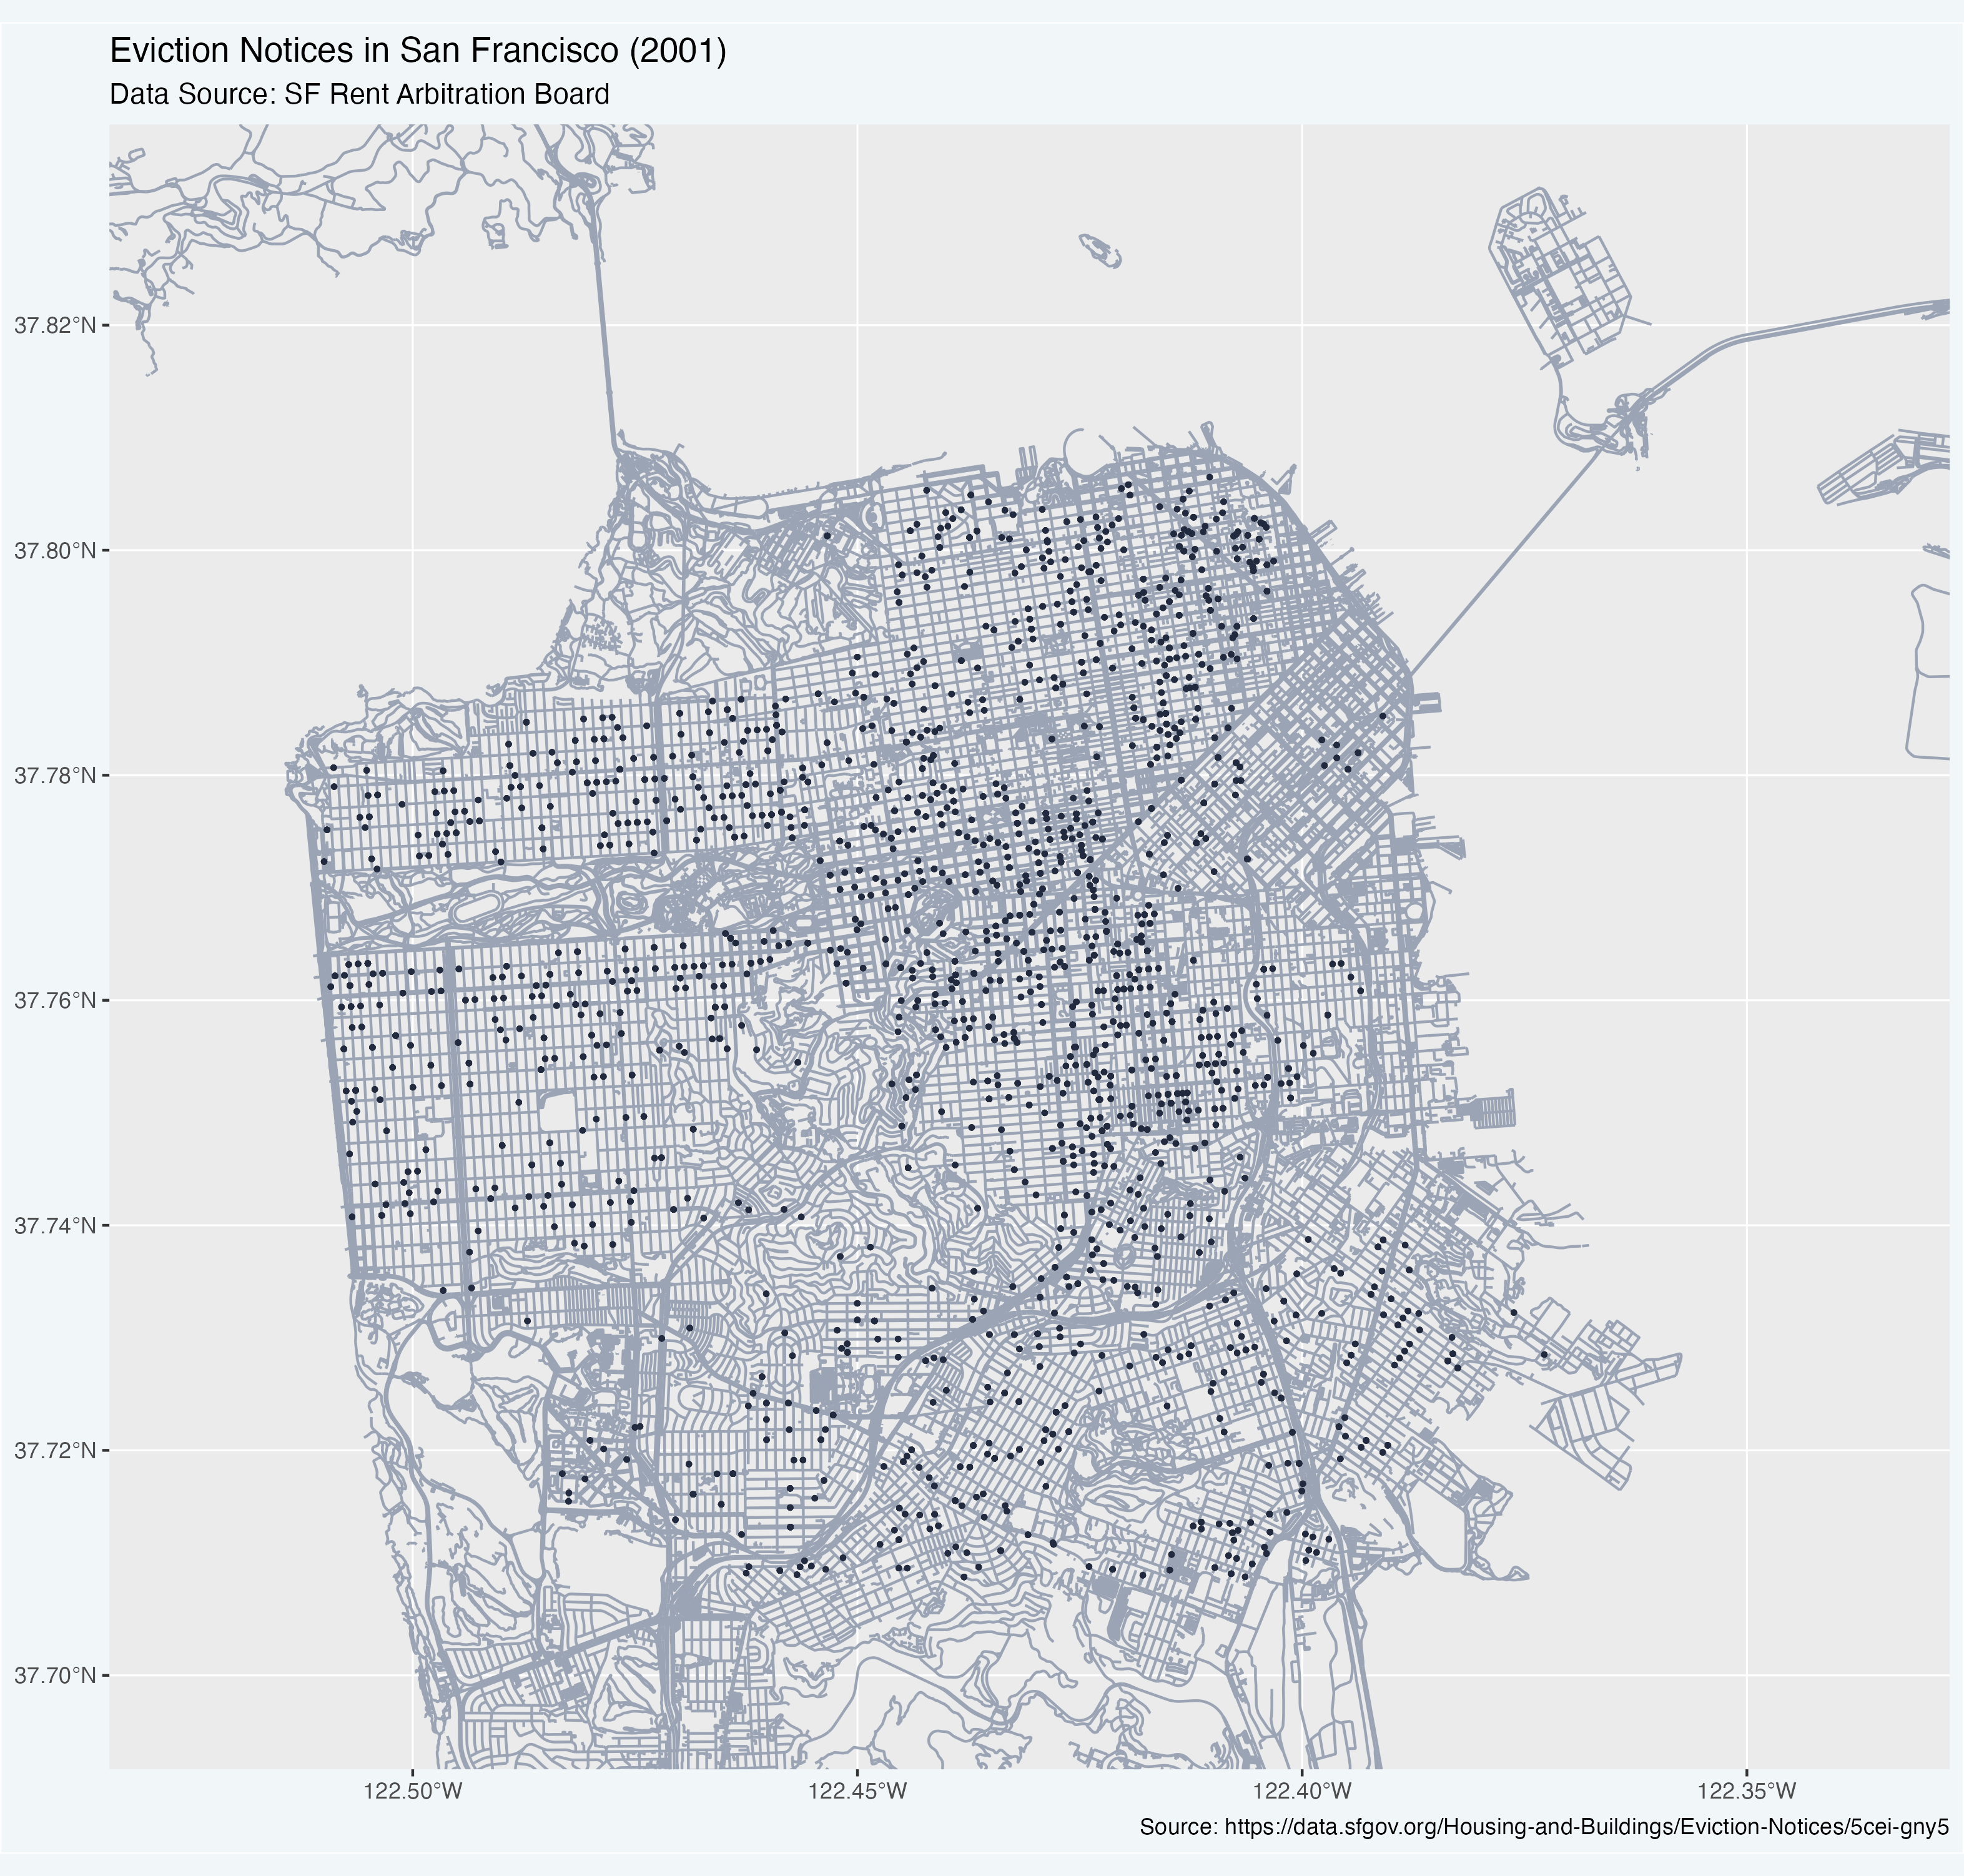
\includegraphics[width=0.3\textwidth]{images/eviction_notices_by_year/2001.png}}
    \subfigure[Notices in 2002]{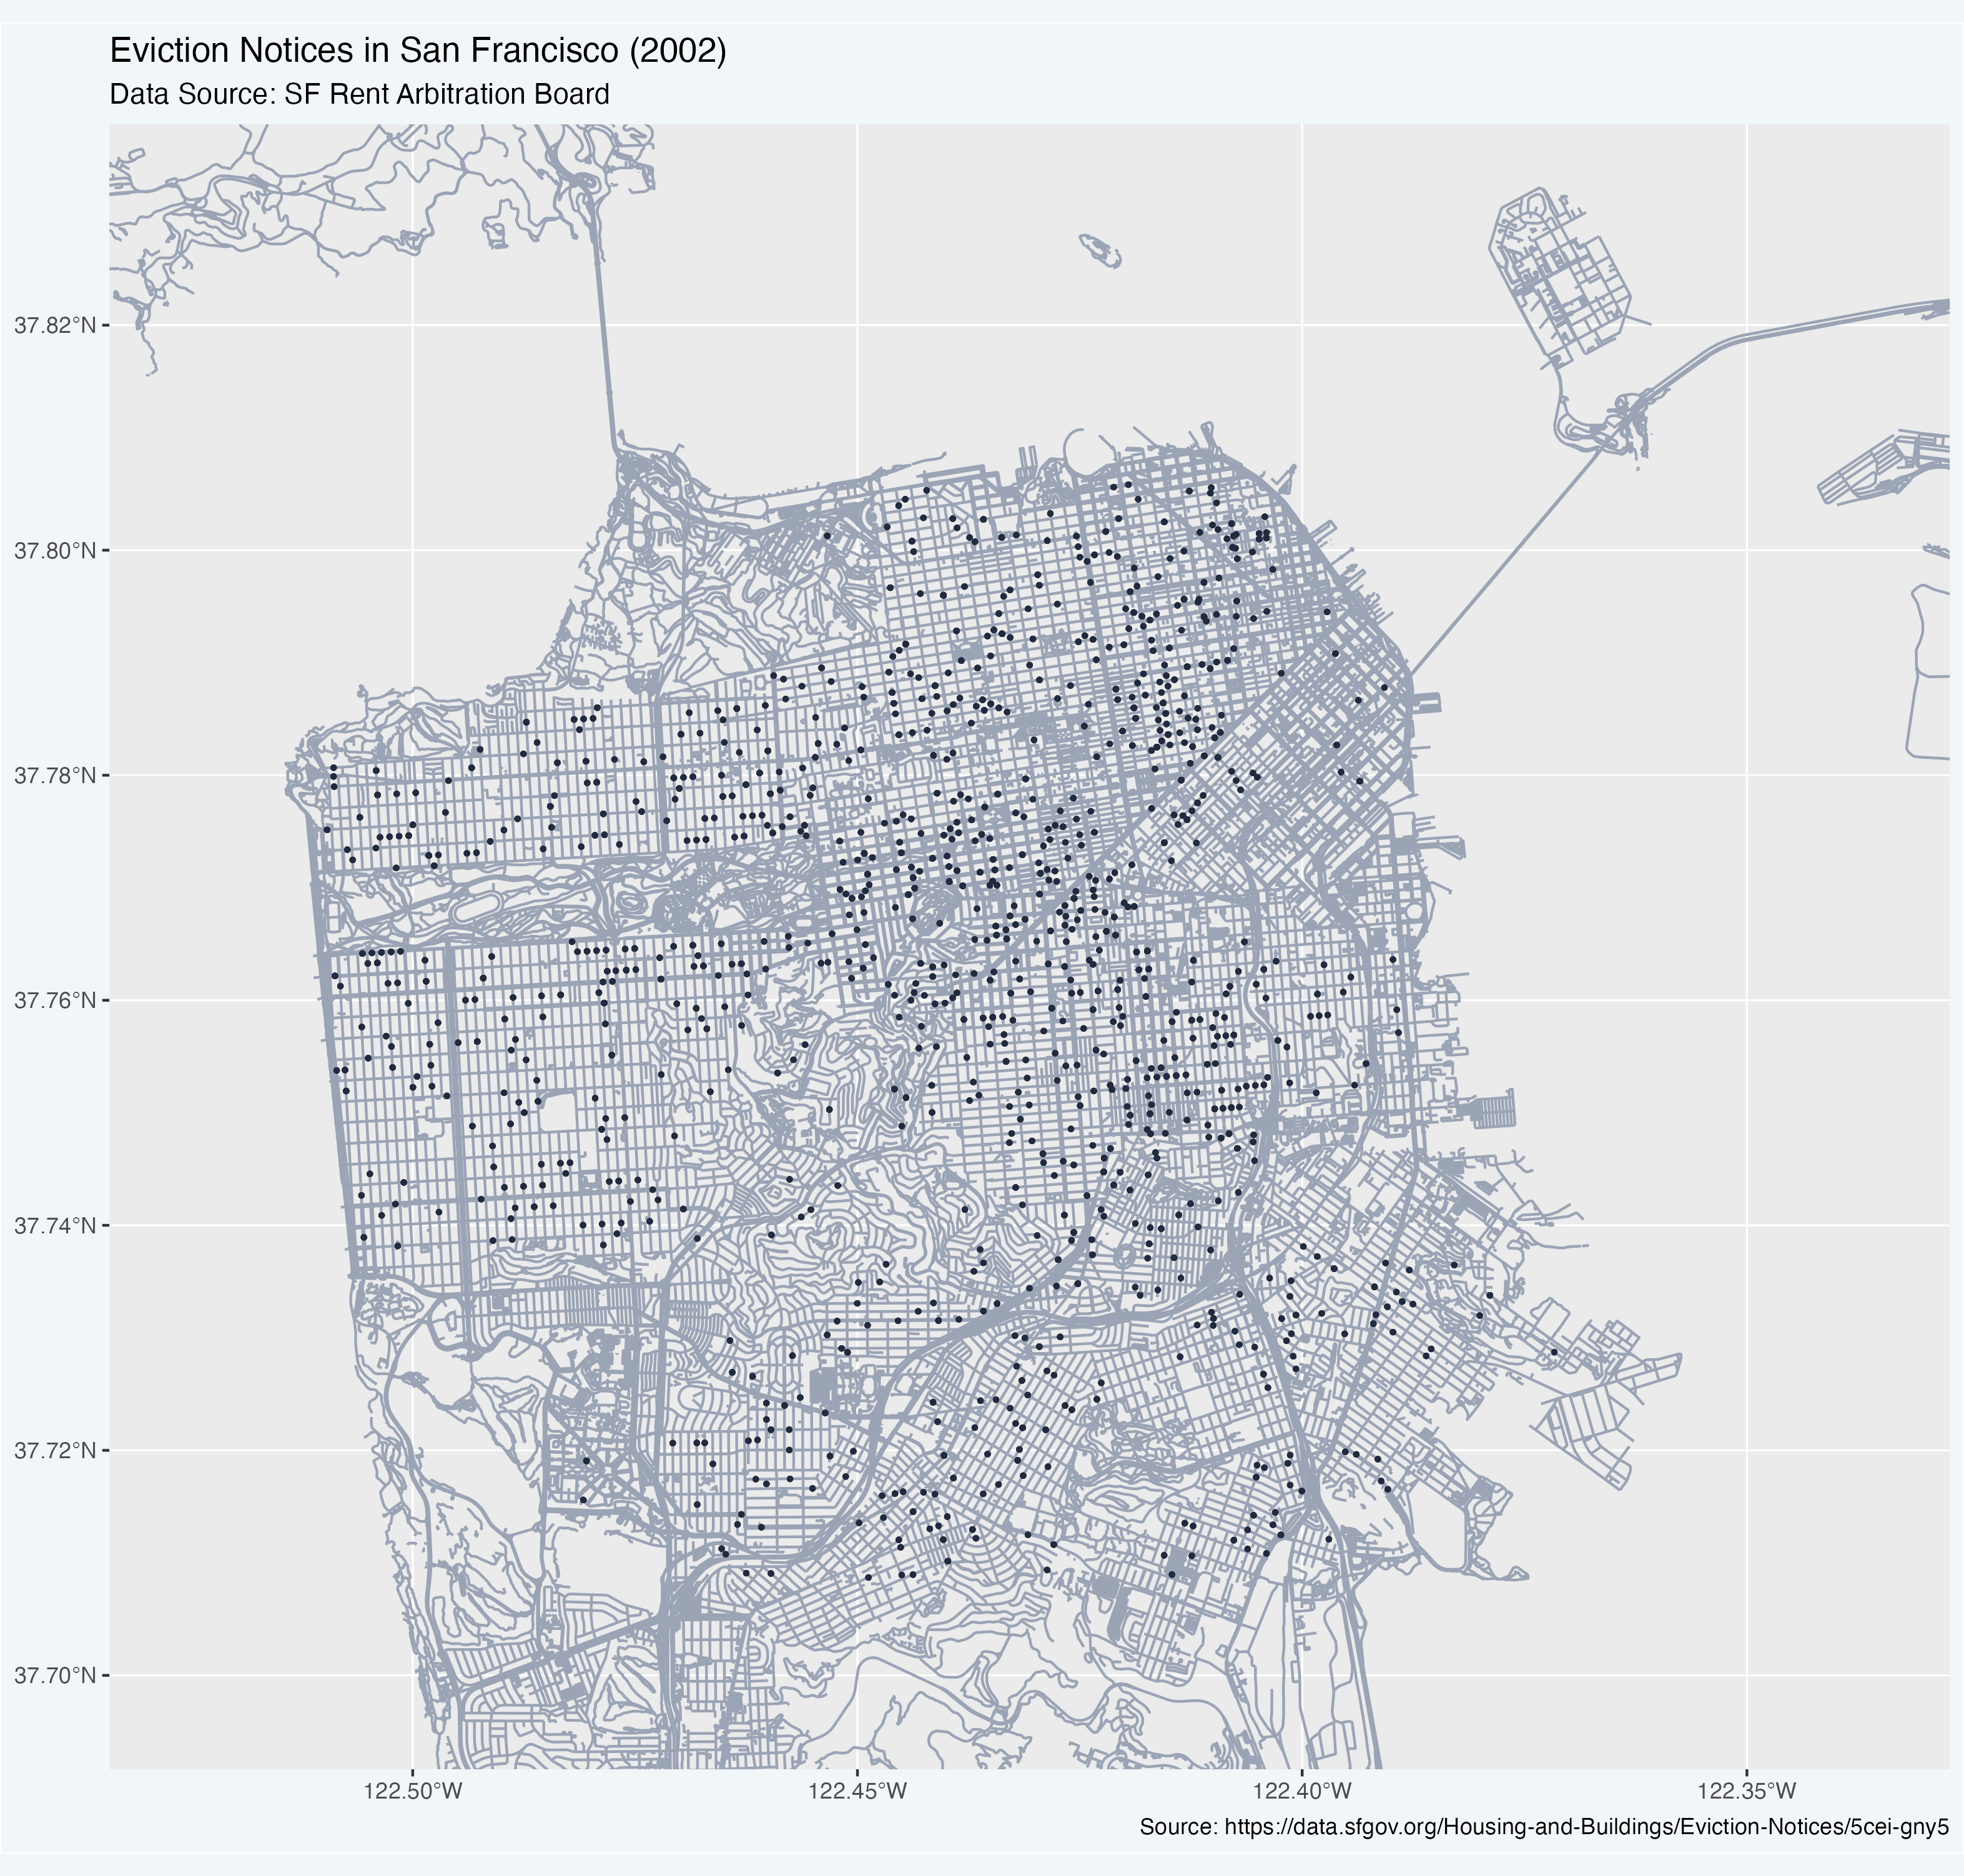
\includegraphics[width=0.3\textwidth]{images/eviction_notices_by_year/2002.png}}
    \subfigure[Notices in 2003]{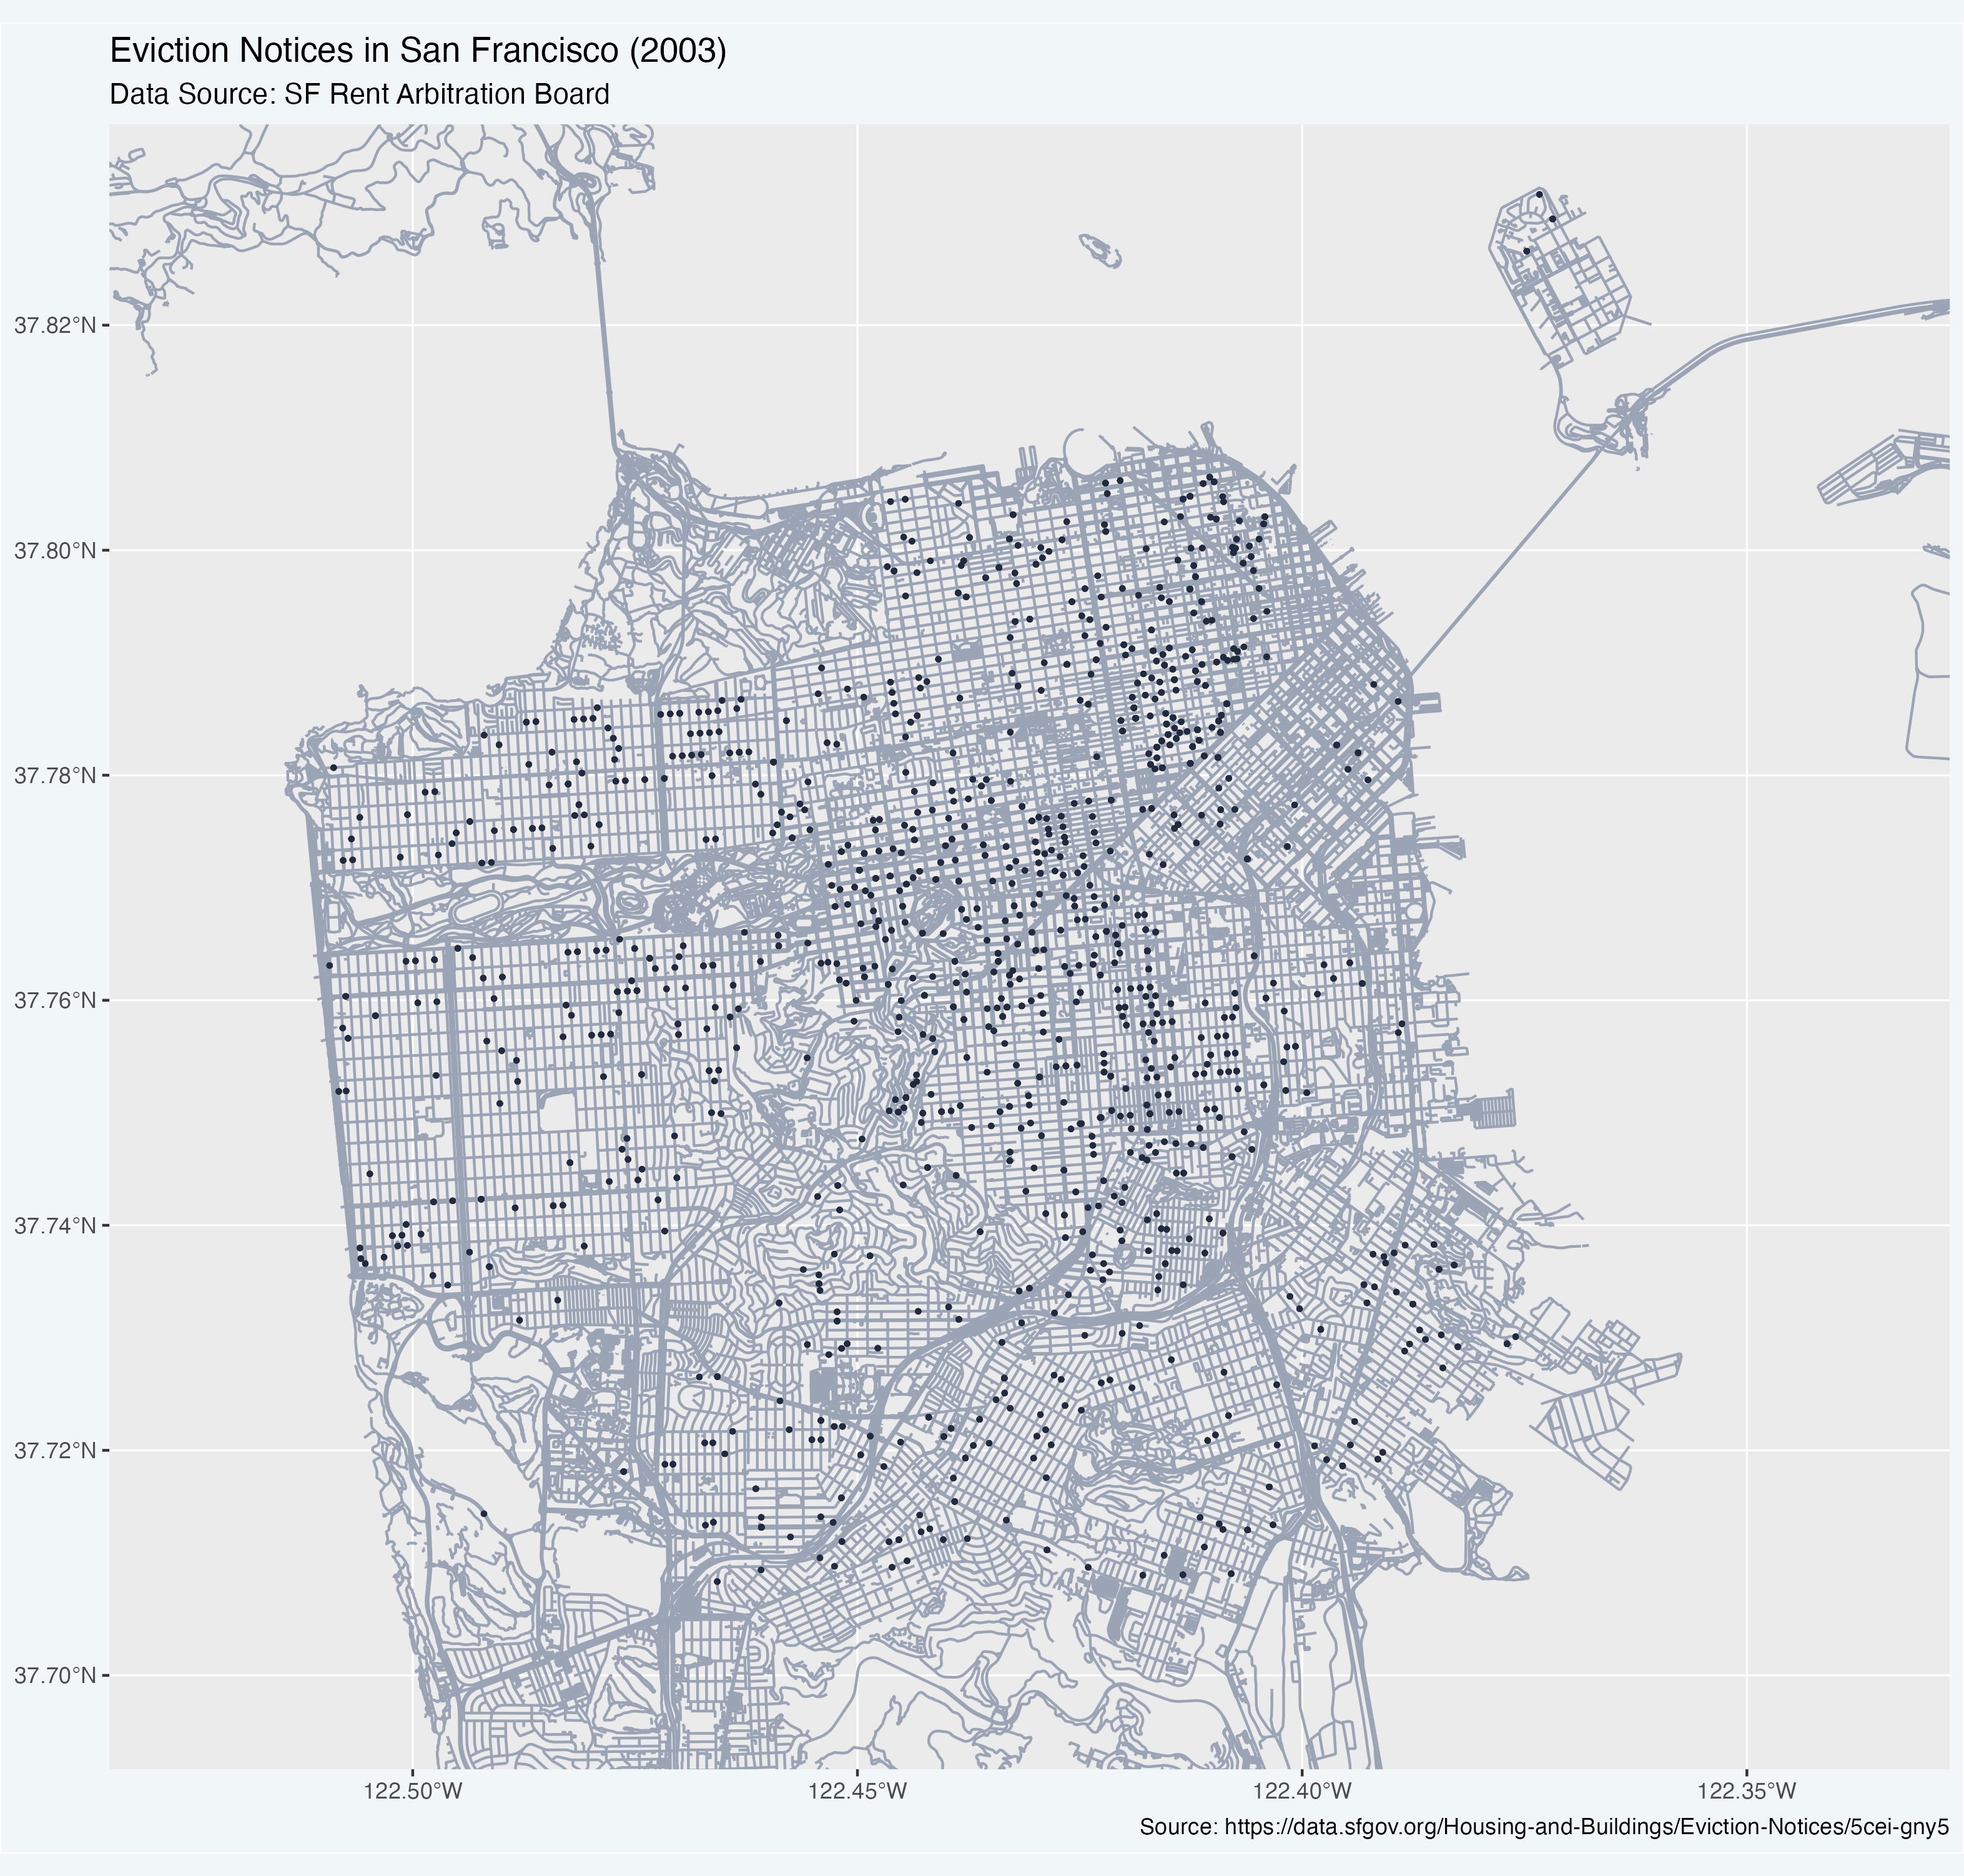
\includegraphics[width=0.3\textwidth]{images/eviction_notices_by_year/2003.png}}
    \subfigure[Notices in 2004]{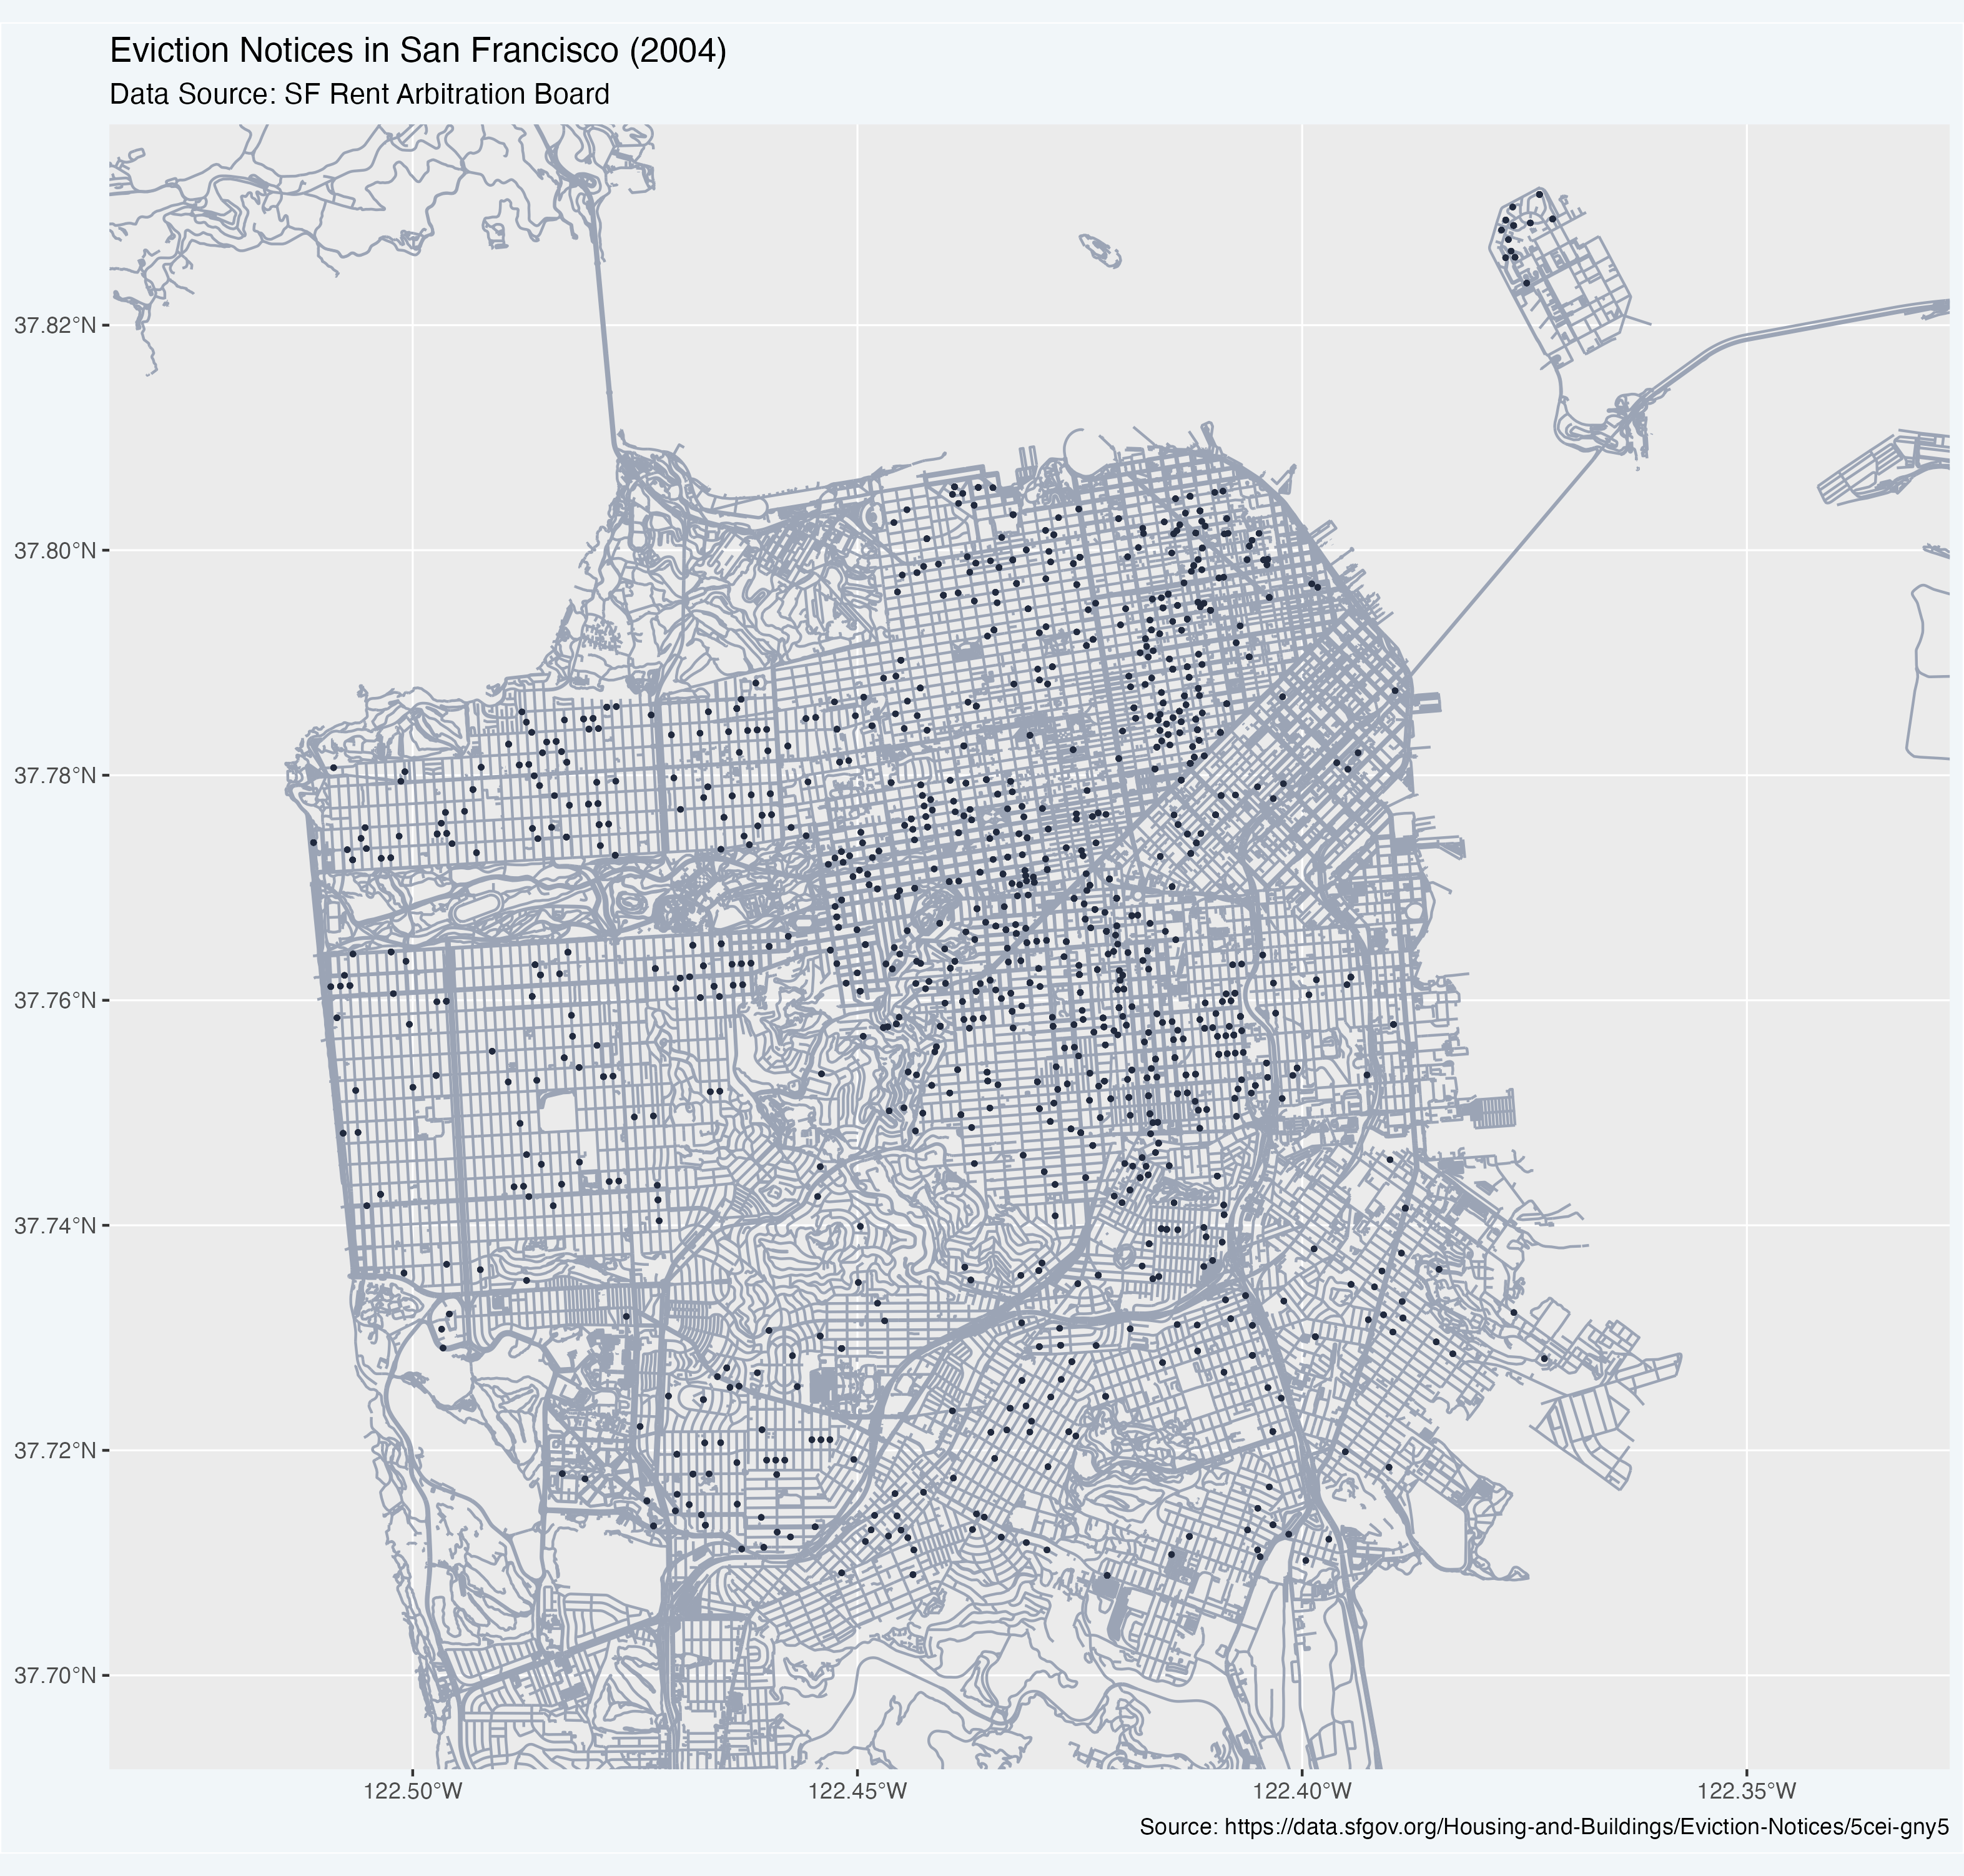
\includegraphics[width=0.3\textwidth]{images/eviction_notices_by_year/2004.png}}
    \subfigure[Notices in 2005]{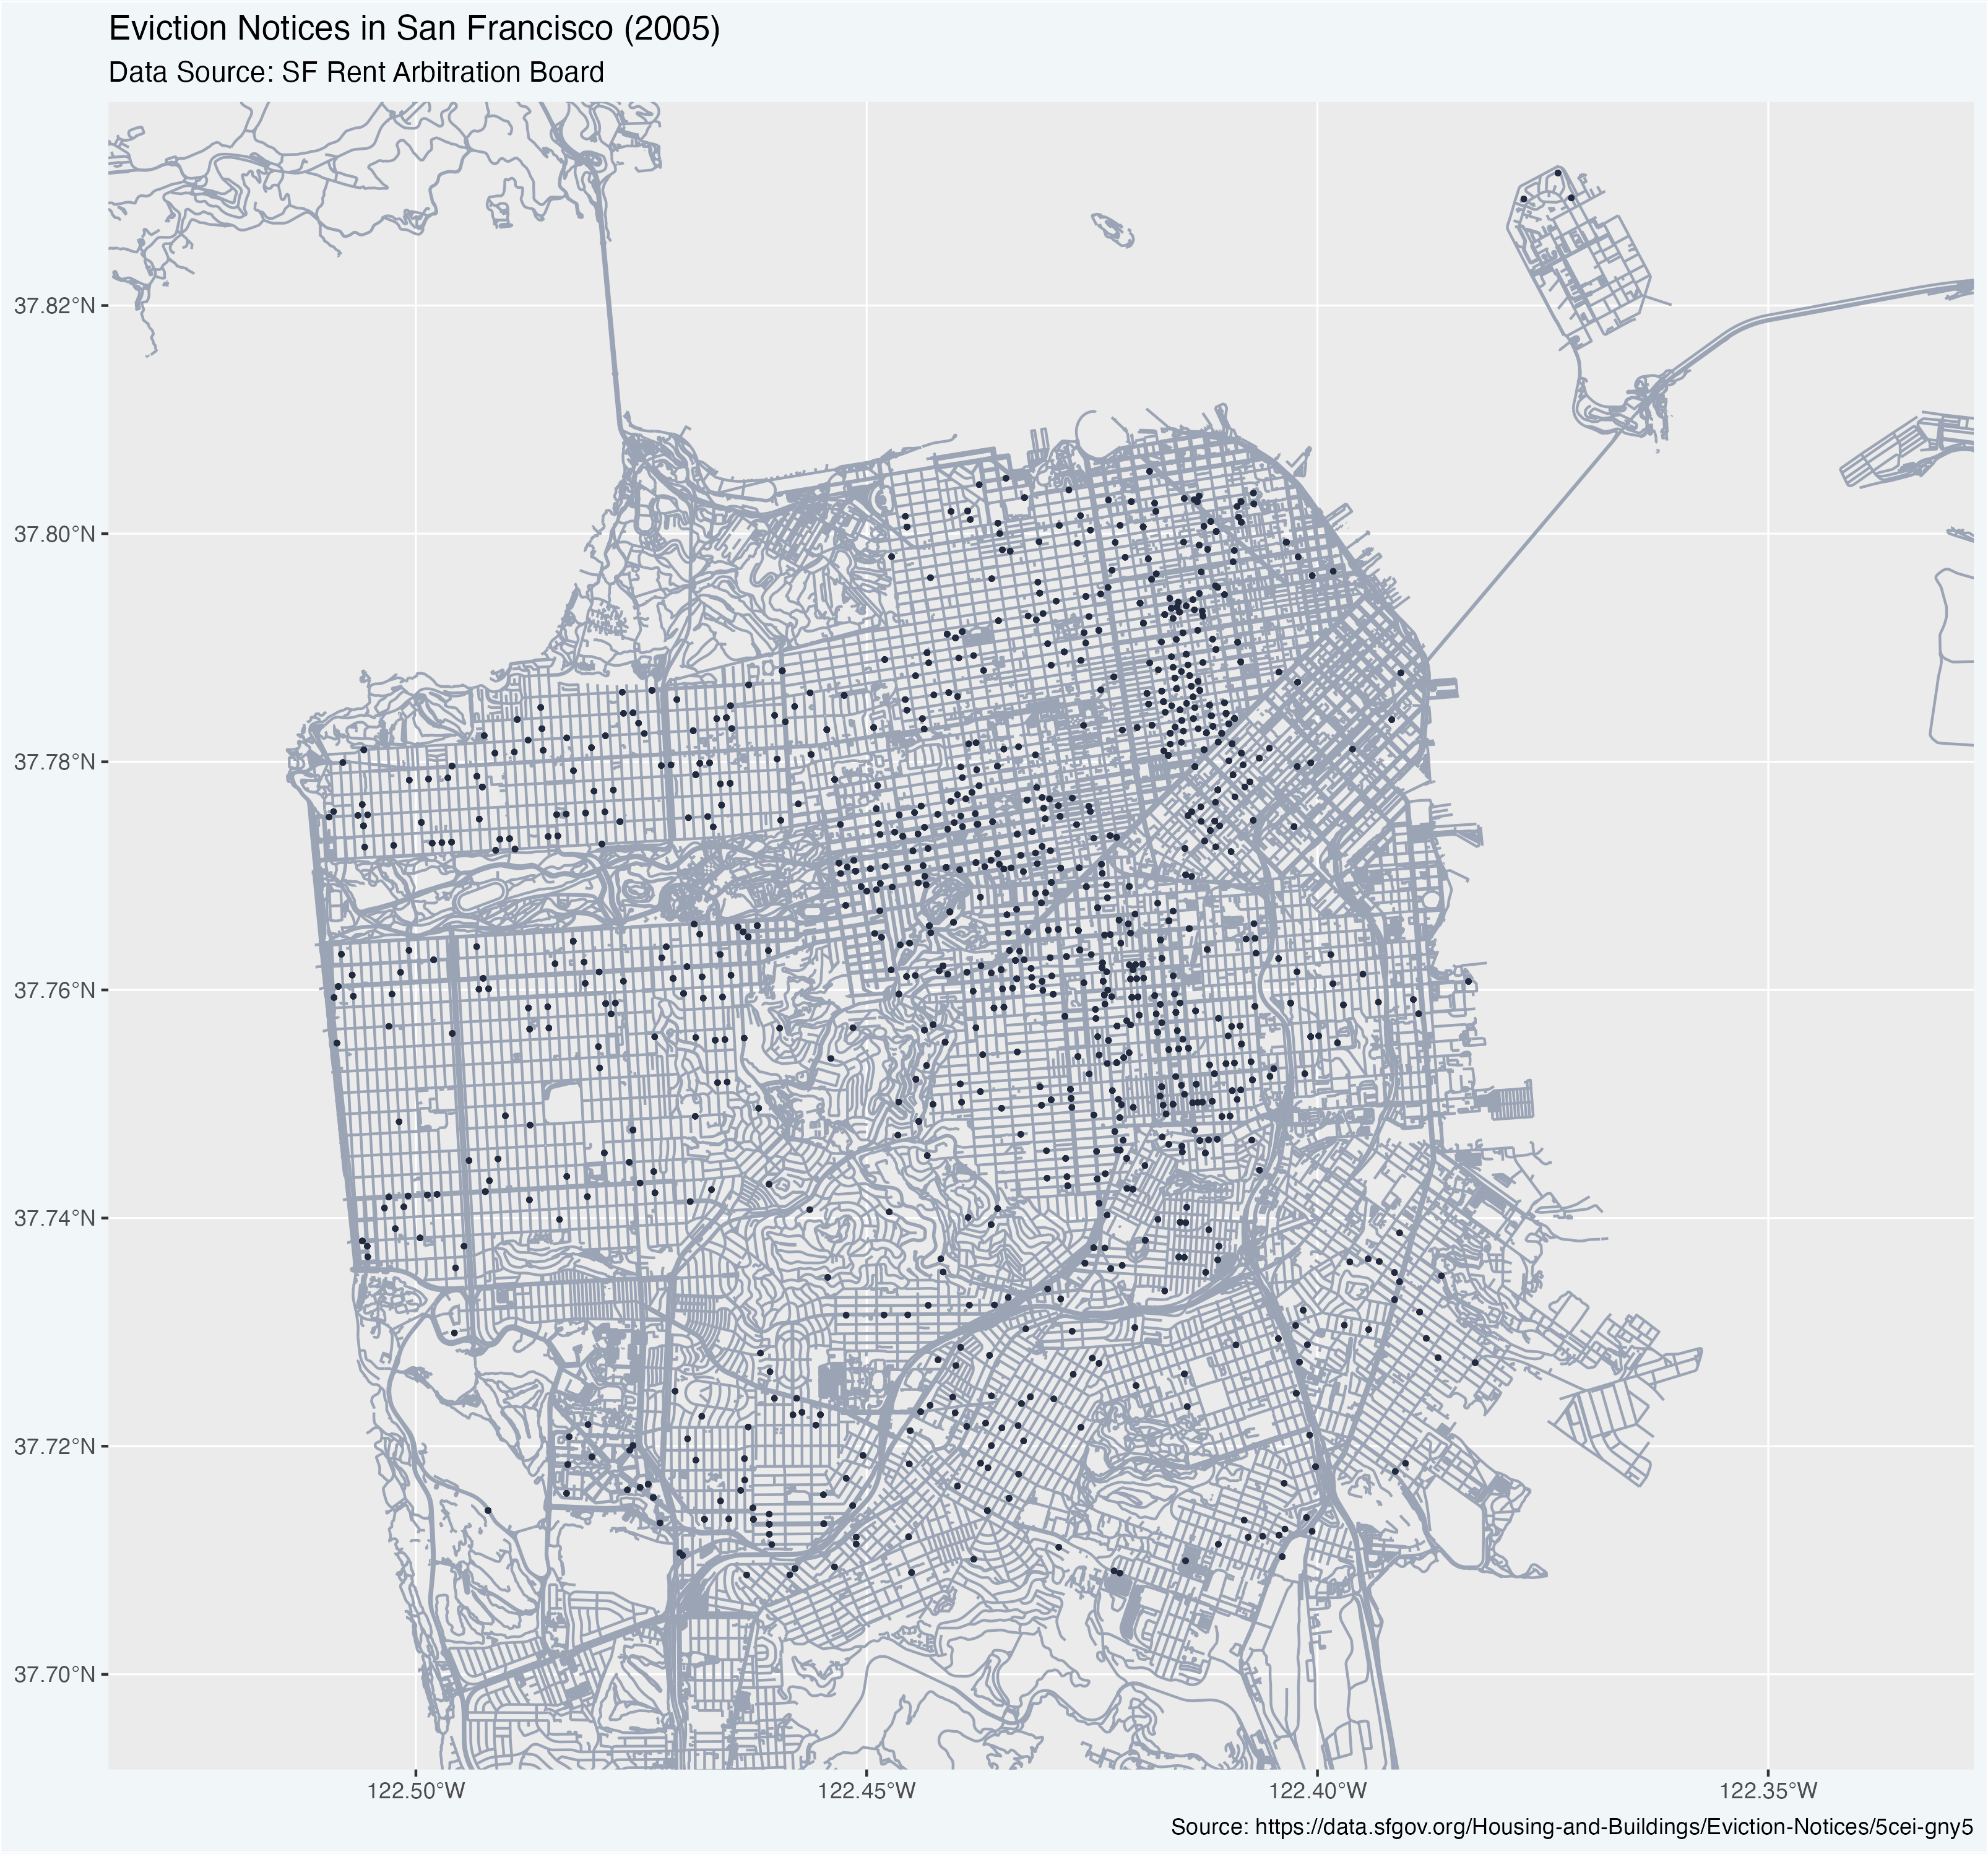
\includegraphics[width=0.3\textwidth]{images/eviction_notices_by_year/2005.png}}
    \subfigure[Notices in 2018]{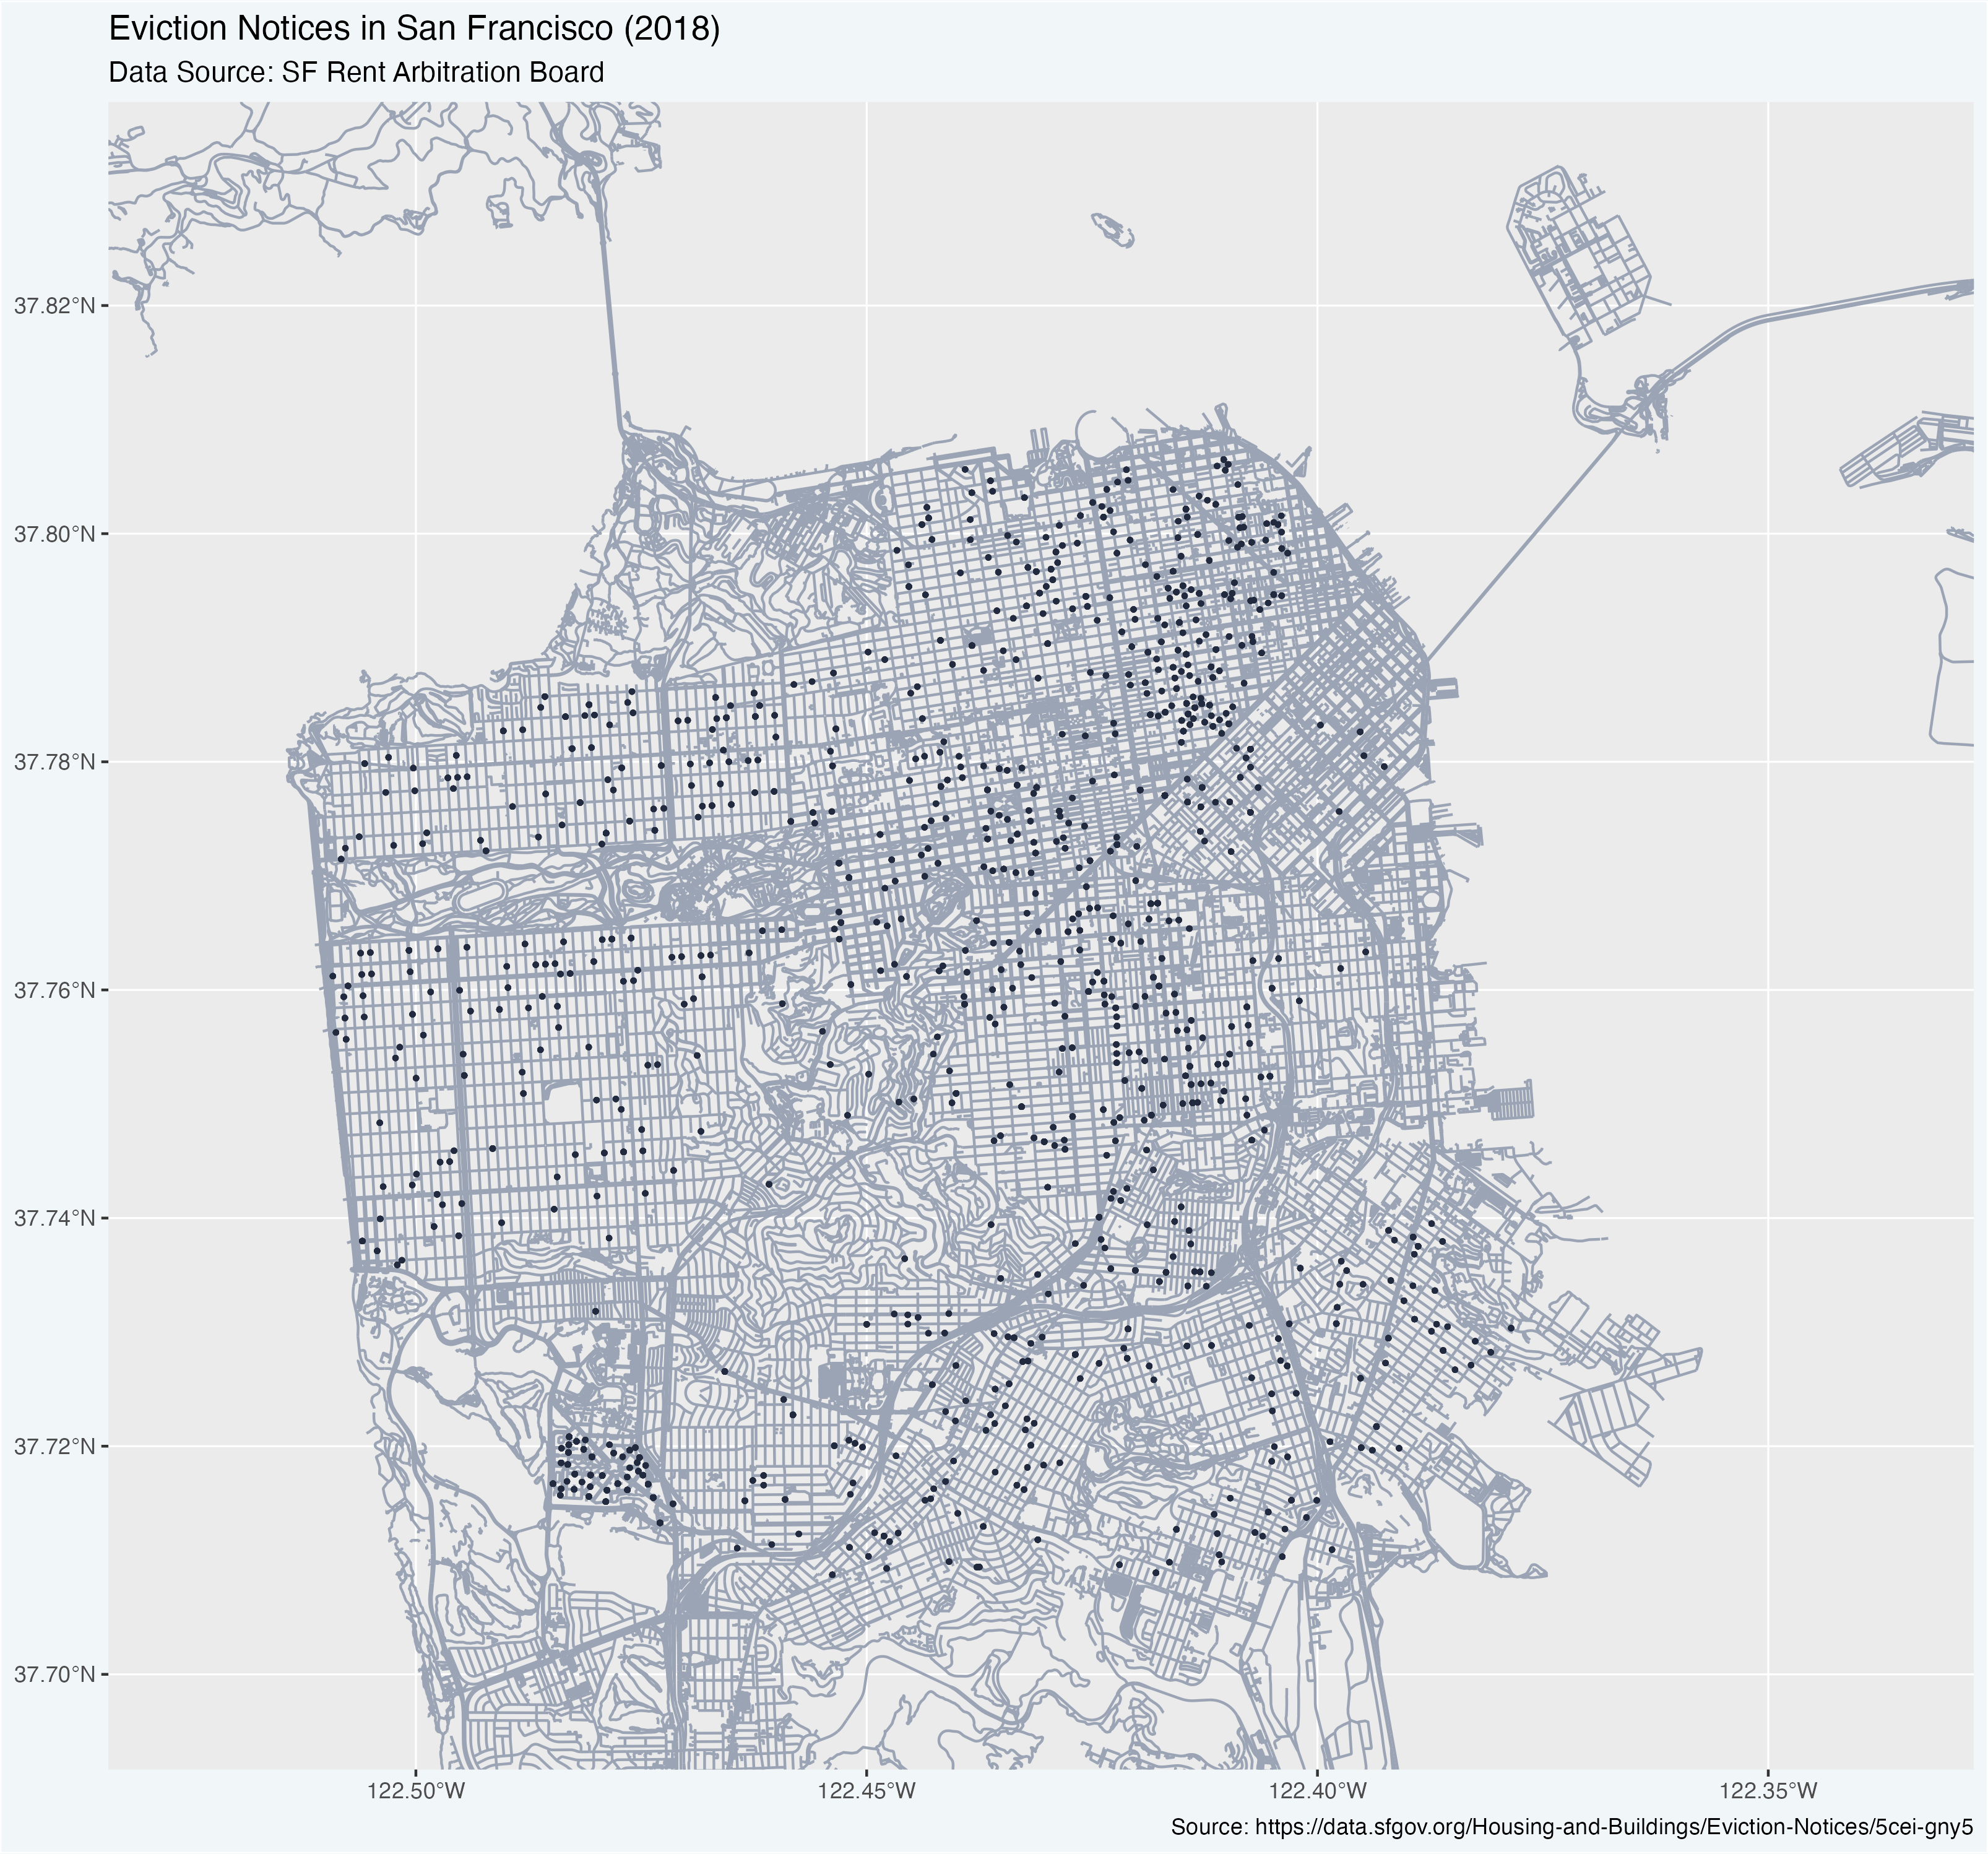
\includegraphics[width=0.3\textwidth]{images/eviction_notices_by_year/2018.png}}
    \subfigure[Notices in 2019]{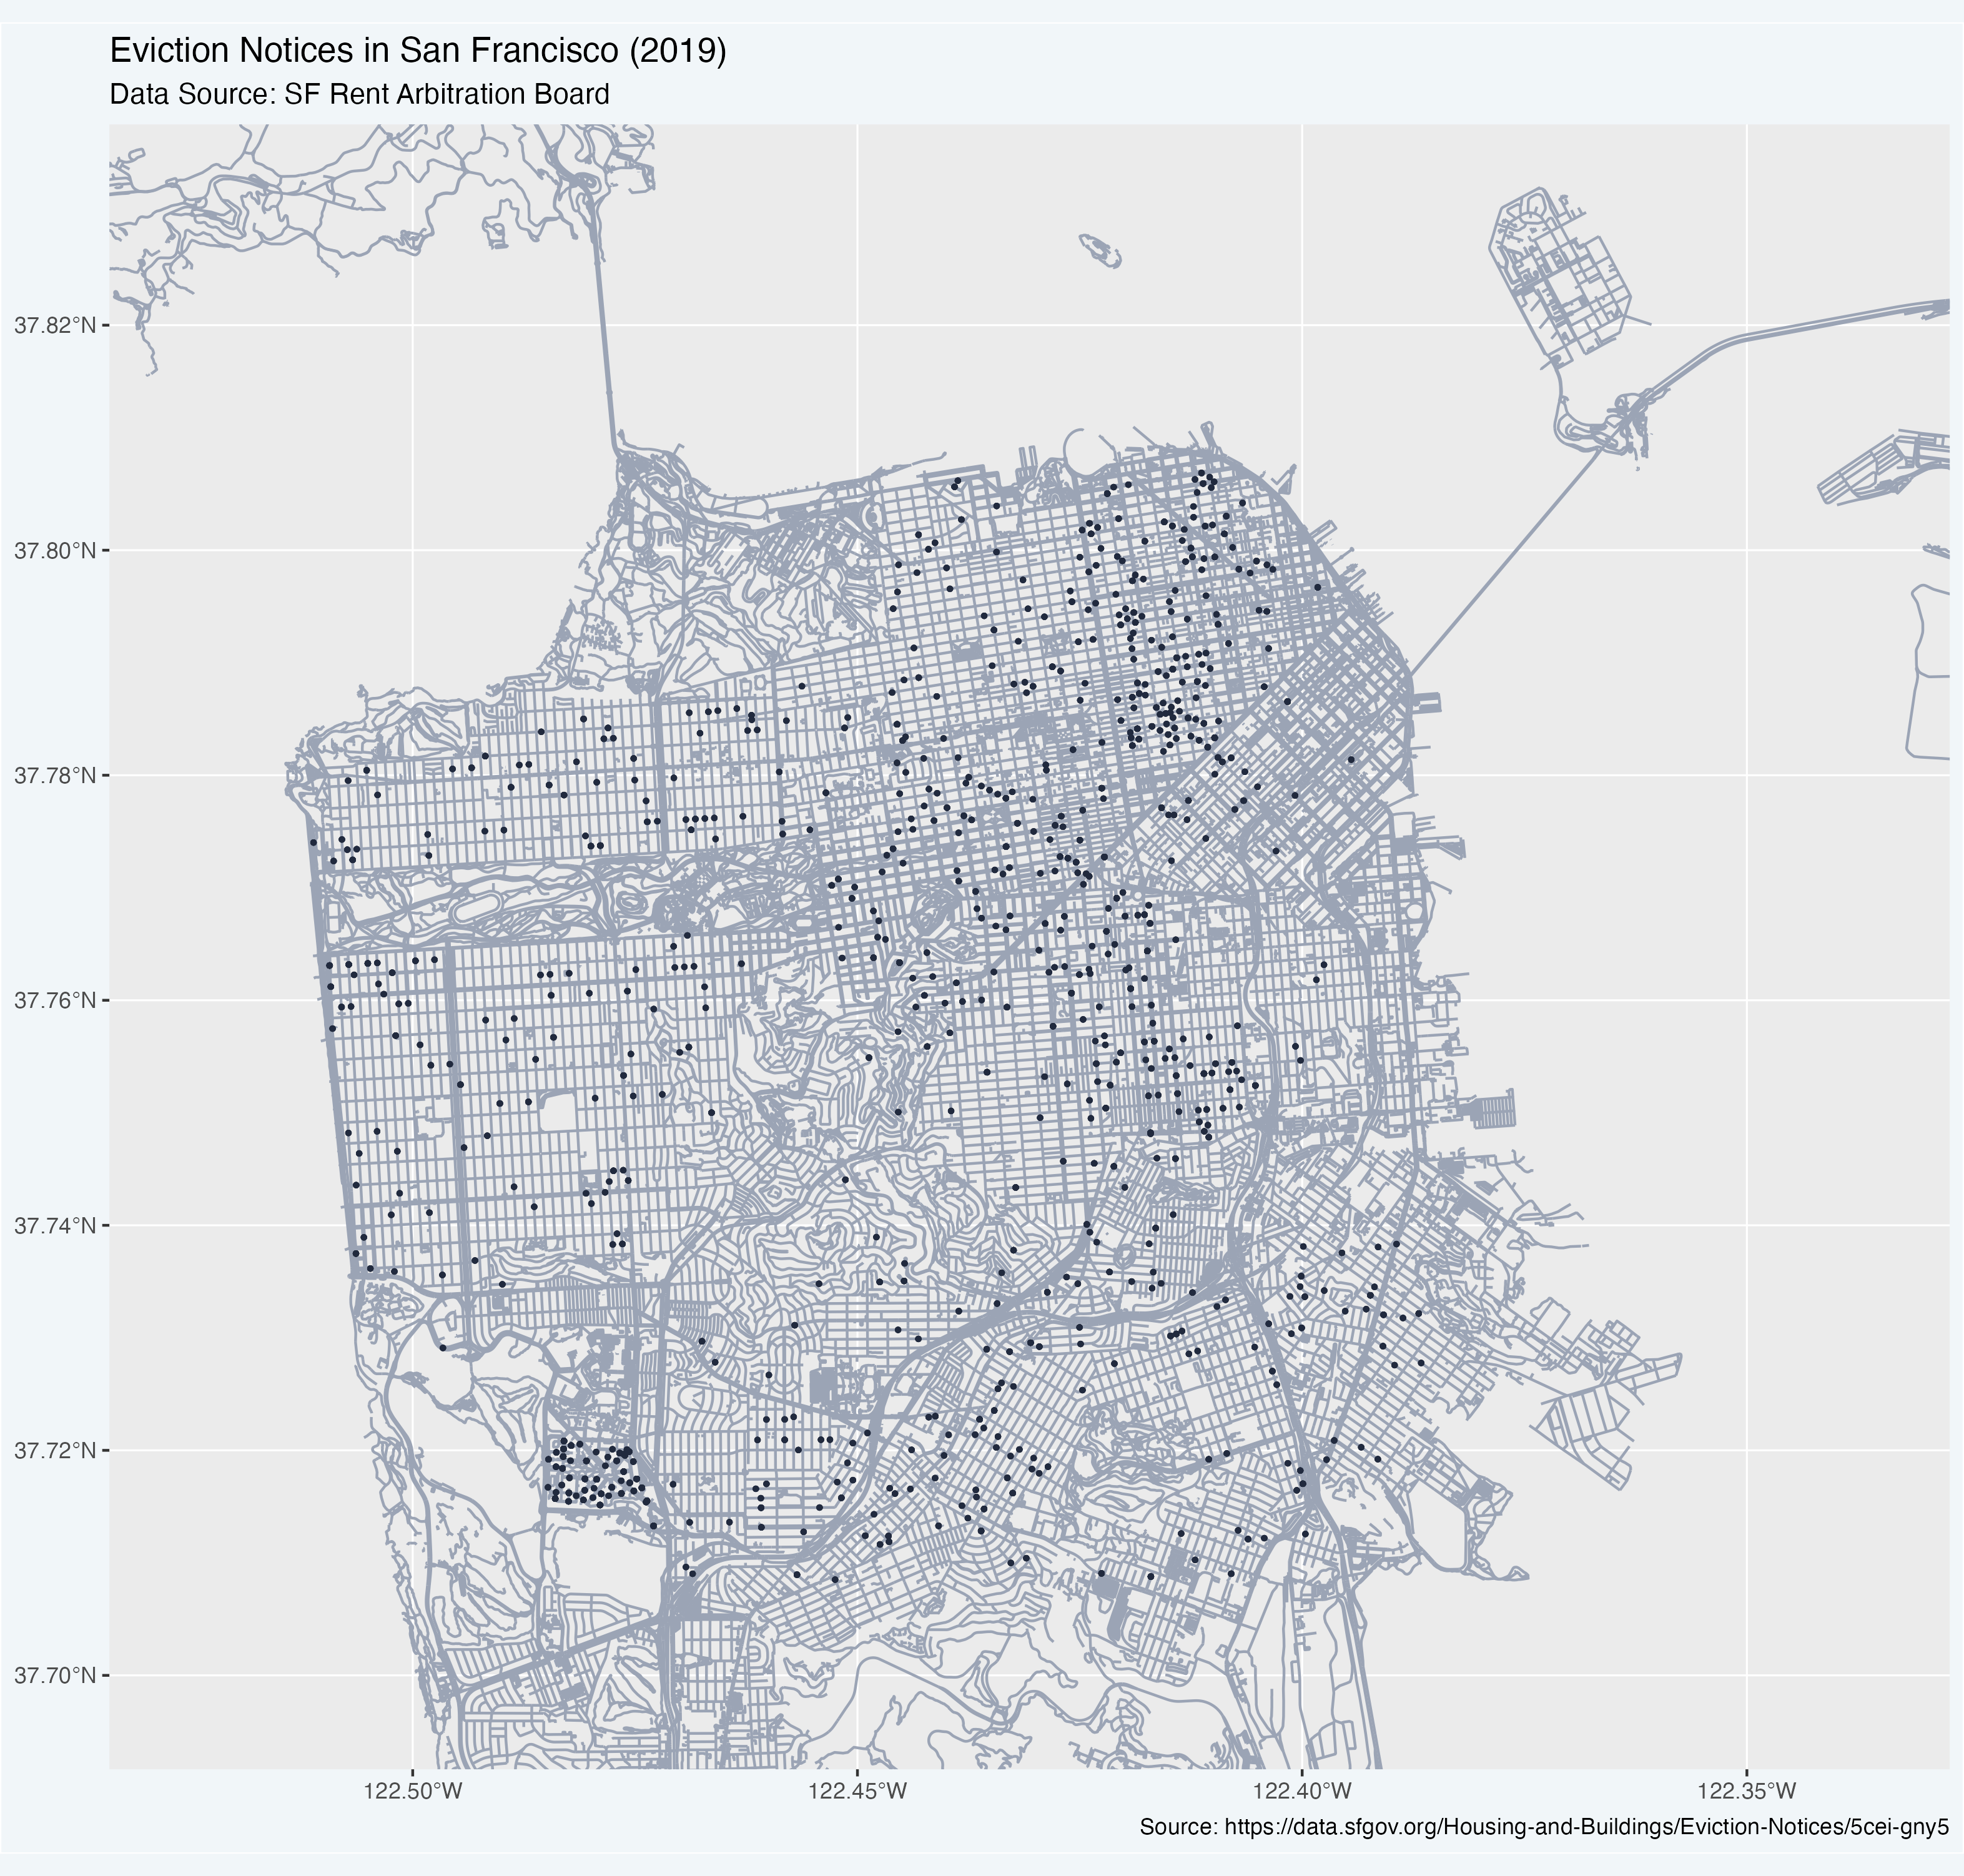
\includegraphics[width=0.3\textwidth]{images/eviction_notices_by_year/2019.png}}
    \subfigure[Notices in 2020]{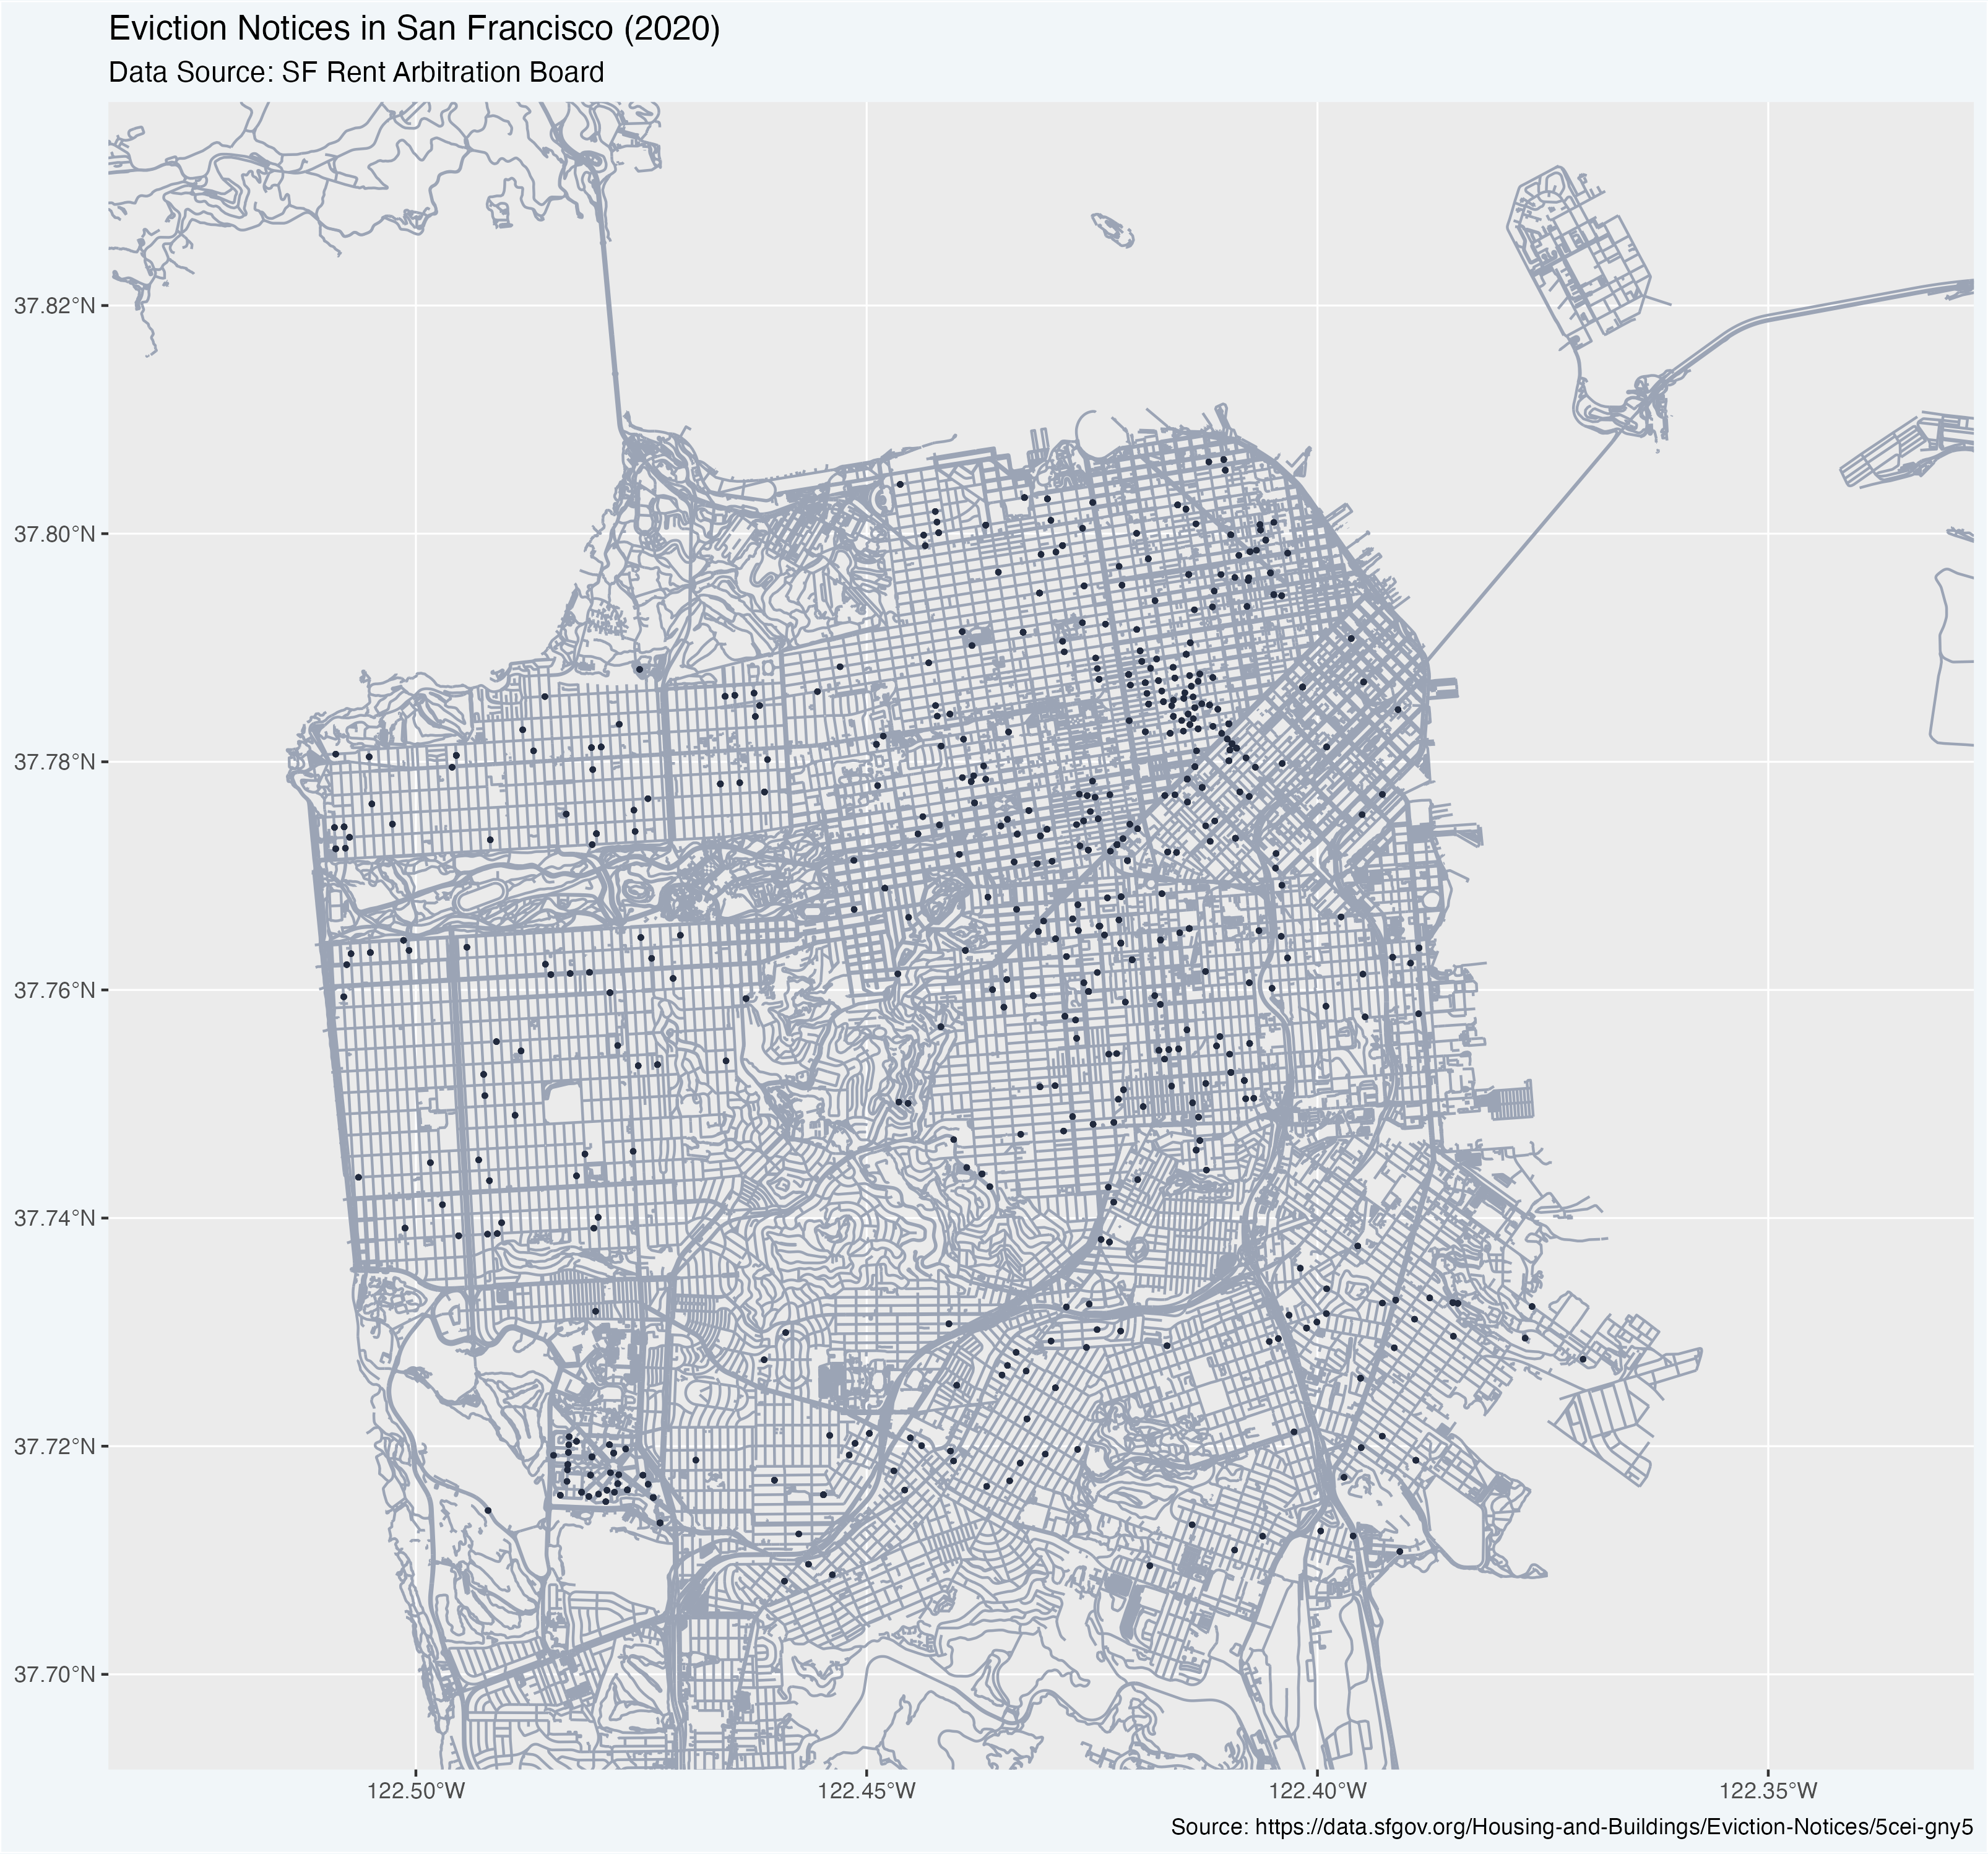
\includegraphics[width=0.3\textwidth]{images/eviction_notices_by_year/2020.png}}
    \caption{Eviction notices by year (1997-2005, 2018-2020)}
    \label{fig:images}
\end{figure}

I first plotted the evictions onto a map of San Francisco by year (FD), to both get a sense of the changes in frequencies of evictions and the actual locations of evictions. The density of evictions in the late 1990's was much higher than subsequent years and they were mostly concentrated in the Mission District and Tenderloin, both of which are neighborhoods that suffered from historic redlining (a discriminatory practice that denies services such as a loan or mortgages to minority communities marked as inadequate or risks).

The effect of redlining and historic discrimatory practices is highlighted in this graph, and the evictions continue staying concentrated in those areas onward past the 1990s. One of the devastating consequences of these historic practices is that there is a dispraportionate amount of minority groups that are evicted because they have effectively been pushed into these neighborhoods.

One other thing to note is that the periodic clusters of eviction notices in the bottom left corner in the neighborhood, Parkmerced. This large, single-owner neighborhood complex has been under scrutiny for sudden evictions as it prepares for new development projects and renovations.

\pagebreak

\subsection{Seasonal Changes}
Organizing evictions by seasons using FD allows us to see if there are any seasonal trends in evictions. Winter evictions are significantly lower than the other seasons. I have not found a solid reason from research but it can be a combination of increased rent protections.

Evictions by season:
\begin{enumerate}
    \item Spring: 45872
    \item Summer: 47528
    \item Fall: 44048
    \item Winter: 12126
\end{enumerate}


\subsection{Plotting Counts by Year and Month}
Organizing the frequencies of counts by year and months allows for a clear picture on how evictions have been trending. There are two distinct spikes: the period around the "dot-com boom/bubble burst" and the beginning of the 2010s, when the real estate market was growing. It is interesting to note that during the "Internet boom" (1998-99), evictions were at the all time high in this data set because of a frenzy to capture the "'new money' that arrived during the 1990s. The fabled boom-time economy, fueled by the dot.com explosion, cannibalized the housing stock and the last blue-collar jobs."

The second spike in the early 2010s is a result of the real estate market growing after the 2008 recession. One interesting finding I found as a result of research into this is that landlords seek to evict more people when they know they can profit the most, which would mean a growing market.

For the plot of counts by month, I added a LOESS regression curve to show a general trend of evictions. I used GGPlot2's loess curve from the \emph{geom\_smooth} function.

\subsection{Zooming into the Spikes: Owner Move-In and Ellis Act Evictions}
I then looked at two common ETs: owner move-in (OMI) and Ellis Act evictions (EAW). Owner move-in evictions are when the landlord evicts the tenant to move themself or relatives into the unit. Ellis Act Withdrawal evictions are when the landlord evicts the tenant to remove the unit from the rental market. I plotted the evictions by year and by neighborhood to see if there were any trends in the data.

OMI evictions make up a significant amount of the evictions, and it peaks in the late 1990's before significantly decreasing starting in 1998, when EAW evictions began increasing shortly afterwards. This trend comes from the abuse of OMI evictions as a way to clear multifamily buildings, and it was rampantly used until a reform effort passed by Sue Bierman to restrict the number of OMI evictions in a building. EAW evictions then began rising as a result of the tech bubble burst and maintained consistent even after that period. Tied with the mapping of evictions above, the neighborhoods that are most affected by OMI and EAW evictions are the Mission District and the Tenderloin.


\section{A Great Recession, a Tech Boom, and a Pandemic}
The time period between 2009-2023 is interesting because while the LOESS curve generally followed the evictions before well, it overpredicts the evictions at the start of this time period, underpredicts the evictions in the middle, and does a mix of both at the end. I now bound the scope of this paper to this time period to explore the changes in eviction types and strategies.

\subsection{Using a Simple Model to Predict Proportions of ETs}

I used a binomial distribution as a model to calculate the expected proportion of each ET.

Let $R_{t,i}$ be the number of evictions with type $t$ in time period $i$ and $n_i$ be the total number of evictions in time period $i$. Suppose that $R_{t,i} \sim \mathrm{Binomial}(n_i, p_{t,i})$ where $p_{t,i}$ is the proportion of eviction type $t$ in time period $i$. We can construct a likelihood function and find the maximum likelihood equation (MLE) for $p_{t,i}$.

\begin{align*}
    \mathcal{L}(p) &= \prod_{t, i} {\mathrm{Binomial}(R_{t,i} | n_i , p_{t,i})} \\
    \mathcal{L}(p) &= \prod_{t, i} {n_i \choose R_{t, i}} p^{t_i}(1-p_{t,i})^{n_i-R_{t, i}} \\
    \ln\mathcal{L}(p) &= \sum_{t,i} \left( \ln{n_i \choose R_{t, i}} + R_{t, i} \ln p + (n_i-R_{t, i}) \ln (1-p) \right) \\
    \frac{d}{dp} \ell(p) &= \sum_{i=1} \frac{R_{t, i}}{p_{t,i}} - \frac{n_i - R_{t, i}}{1-p_{t,i}} \\
    0 &= \sum_{i=1} \frac{R_{t, i}}{p} - \frac{n_i - R_{t, i}}{1-p_{t,i}} \\
    0 &= \sum_{i=1} R_{t, i} - p_{t,i}\sum_{i=1}^{n} n_i \\
    p &= \frac{\sum_{t, i} R_{t, i}}{\sum_{t, i} n_i} \\
\end{align*}

Using this derived MLE for $\hat{p}$ I can calculate the expected proportion for each ET:

\begin{knitrout}
\definecolor{shadecolor}{rgb}{0.969, 0.969, 0.969}\color{fgcolor}\begin{kframe}
\begin{alltt}
\hlcom{# Calculate the expected proportion for each eviction type}
\hlstd{calc_proportions} \hlkwb{<-} \hlkwa{function}\hlstd{(}\hlkwc{data}\hlstd{) \{}
  \hlstd{data} \hlopt
    \hlkwd{count}\hlstd{(eviction_type)} \hlopt
    \hlkwd{mutate}\hlstd{(}\hlkwc{prop} \hlstd{= n} \hlopt{/} \hlstd{sum_evictions_09_23)} \hlopt
    \hlkwd{arrange}\hlstd{(eviction_type)}
\hlstd{\}}

\hlcom{# Pass to function then bind data_id which is the period}
\hlstd{e_prop} \hlkwb{<-} \hlkwd{lapply}\hlstd{(evictions_09_23, calc_proportions)}
\hlstd{e_prop} \hlkwb{<-} \hlkwd{bind_rows}\hlstd{(e_prop_tp,} \hlkwc{.id} \hlstd{=} \hlstr{"data_id"}\hlstd{)}

\hlstd{expected_prop} \hlkwb{<-} \hlkwd{sum}\hlstd{(e_prop_tp} \hlopt \hlkwd{pull}\hlstd{(prop))} \hlopt{/} \hlnum{48}
\end{alltt}
\end{kframe}
\end{knitrout}
Where \emph{e\_prop} represents the subsetted data set
$$
\hat{p} = \frac{\sum_{t, i} R_{t, i}}{\sum_{t, i} n_i} = 0.02083333
$$

Plotting this expected value with the observed proportions, we can see that the observed proportions do not agree with the expected proportions almost all of the time; there is a lot of unexplained variation in the data.

\pagebreak
\begin{figure}[htbp]
  \centering
  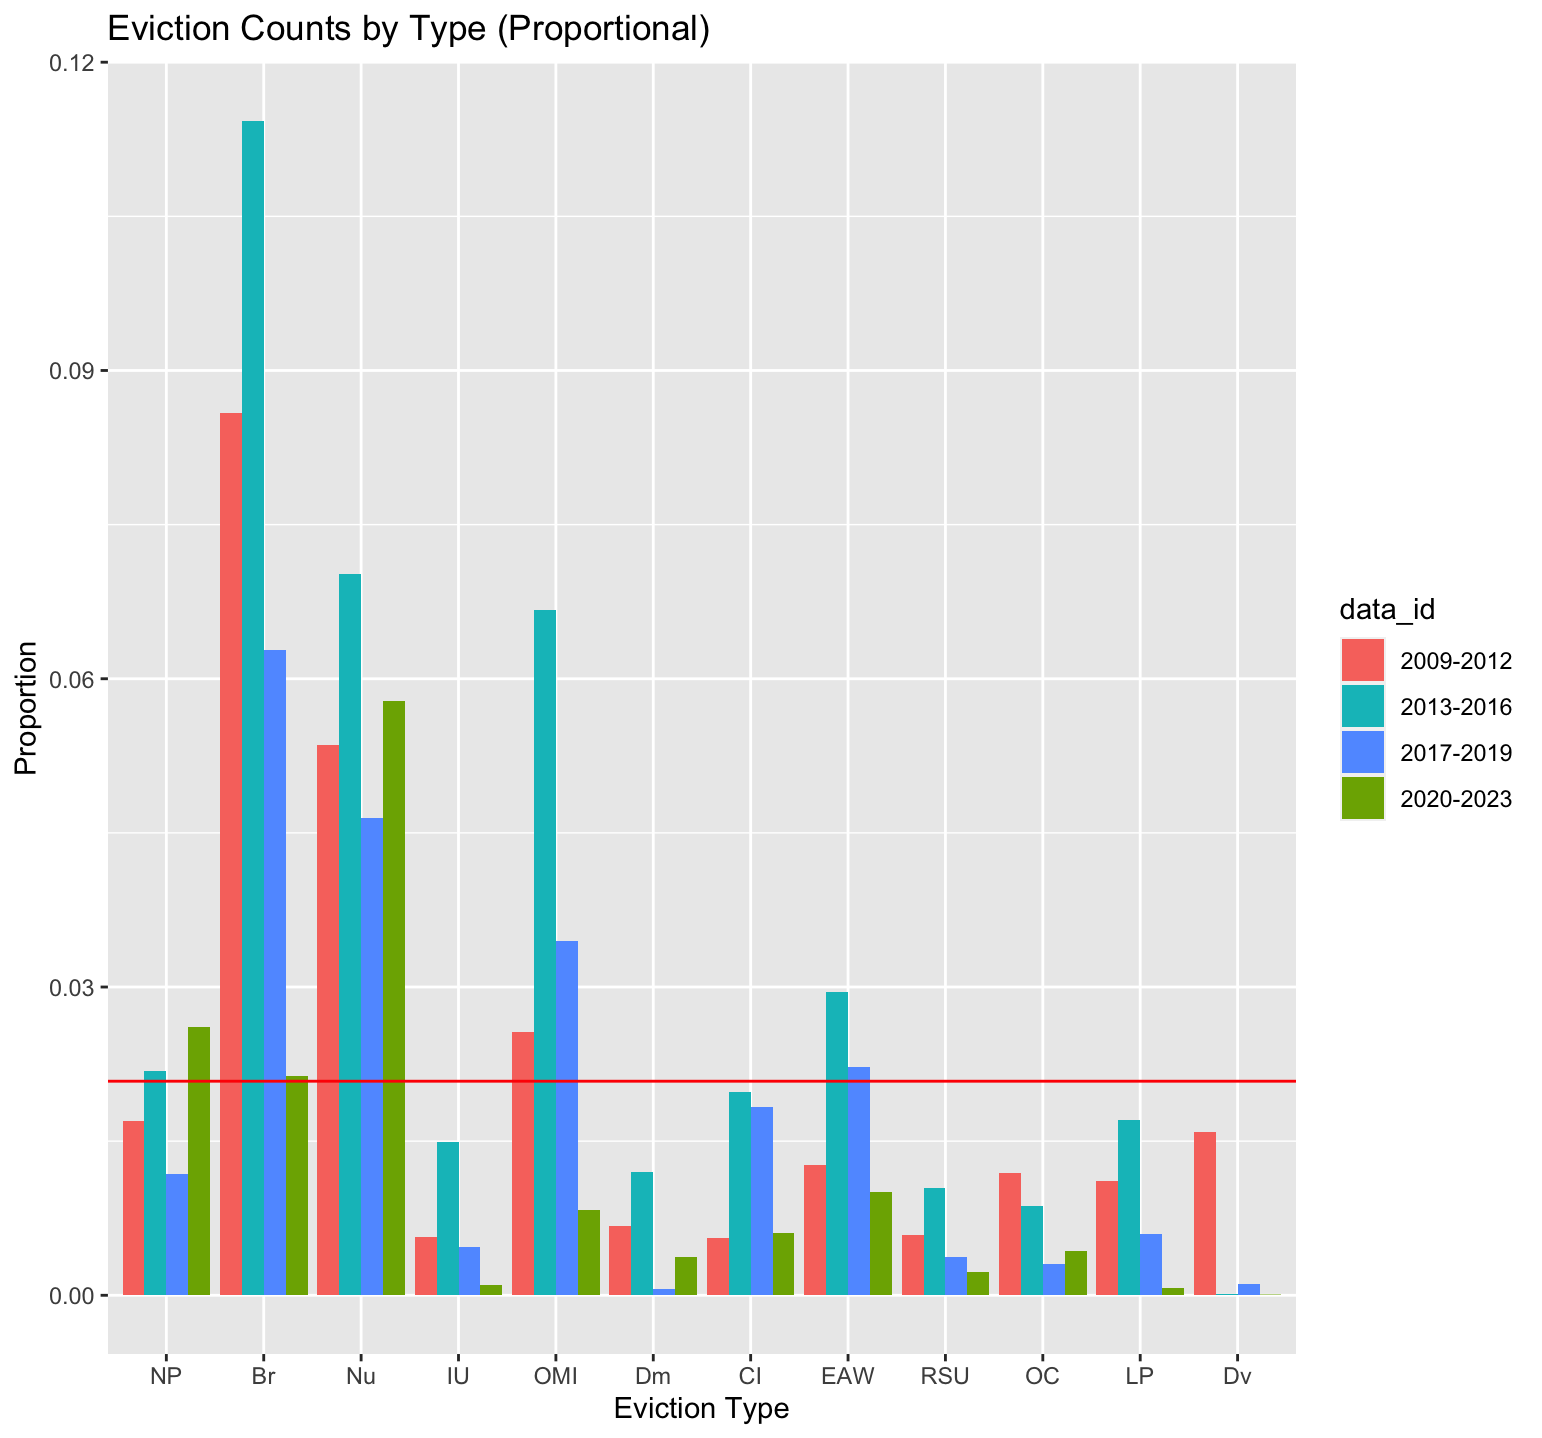
\includegraphics[width=1.\textwidth]{/Users/brianliu03/Documents/Stats2023/data-project/images/counts_tp_prop_ev.png}
  \caption{Proportions of ETs with Expected Value (2009-23)}
  \label{fig:expected_proportions}
\end{figure}
\pagebreak


\subsection{Examining each ET}
I then normalized the proportions of each ET to sum to 1:
\begin{knitrout}
\definecolor{shadecolor}{rgb}{0.969, 0.969, 0.969}\color{fgcolor}\begin{kframe}
\begin{alltt}
\hlstd{e_prop_by_et} \hlkwb{<-} \hlstd{e_prop} \hlopt
  \hlkwd{group_by}\hlstd{(eviction_type)} \hlopt
  \hlkwd{summarize}\hlstd{(}\hlkwc{prop} \hlstd{=} \hlkwd{sum}\hlstd{(prop))}
\end{alltt}
\end{kframe}
\end{knitrout}
and then plotted the proportions of each ET by time period. The data is then bootstrapped, resampling with replacement 10000 times. I then calculated the 99\% confidence intervals for each ET and plotted all of this on a graph.

\begin{knitrout}
\definecolor{shadecolor}{rgb}{0.969, 0.969, 0.969}\color{fgcolor}\begin{kframe}
\begin{alltt}
\hlstd{size} \hlkwb{<-} \hlnum{10000}

\hlstd{get_bs} \hlkwb{<-} \hlkwa{function}\hlstd{(}\hlkwc{size}\hlstd{,} \hlkwc{type}\hlstd{,} \hlkwc{data}\hlstd{) \{}
  \hlcom{# 4 by size matrix, 4 rows for each time period}
  \hlstd{bs_matrix} \hlkwb{<-} \hlkwd{array}\hlstd{(}\hlnum{NA}\hlstd{,} \hlkwc{dim} \hlstd{=} \hlkwd{c}\hlstd{(}\hlnum{4}\hlstd{, size))}

  \hlkwa{for} \hlstd{(i} \hlkwa{in} \hlnum{1}\hlopt{:}\hlstd{size) \{}
    \hlstd{bootstrap_indices} \hlkwb{<-} \hlkwd{sample}\hlstd{(}\hlkwd{seq_len}\hlstd{(}\hlkwd{nrow}\hlstd{(data)),} \hlkwd{nrow}\hlstd{(data),} \hlkwc{replace} \hlstd{=} \hlnum{TRUE}\hlstd{)}
    \hlstd{bootstrap_sample} \hlkwb{<-} \hlstd{data[bootstrap_indices, ]}

    \hlstd{bs} \hlkwb{<-} \hlstd{bootstrap_sample} \hlopt
      \hlkwd{filter}\hlstd{(eviction_type} \hlopt{==} \hlstd{type)}

    \hlstd{e_09_12_bs} \hlkwb{<-} \hlstd{bs[bs}\hlopt{$}\hlstd{File.Date} \hlopt{>=} \hlkwd{as.Date}\hlstd{(}\hlstr{"2009-01-01"}\hlstd{)} \hlopt{&}
      \hlstd{bs}\hlopt{$}\hlstd{File.Date} \hlopt{<=} \hlkwd{as.Date}\hlstd{(}\hlstr{"2012-12-31"}\hlstd{), ]}
    \hlstd{e_13_16_bs} \hlkwb{<-} \hlstd{bs[bs}\hlopt{$}\hlstd{File.Date} \hlopt{>=} \hlkwd{as.Date}\hlstd{(}\hlstr{"2013-01-01"}\hlstd{)} \hlopt{&}
      \hlstd{bs}\hlopt{$}\hlstd{File.Date} \hlopt{<=} \hlkwd{as.Date}\hlstd{(}\hlstr{"2016-12-31"}\hlstd{), ]}
    \hlstd{e_17_19_bs} \hlkwb{<-} \hlstd{bs[bs}\hlopt{$}\hlstd{File.Date} \hlopt{>=} \hlkwd{as.Date}\hlstd{(}\hlstr{"2017-01-01"}\hlstd{)} \hlopt{&}
      \hlstd{bs}\hlopt{$}\hlstd{File.Date} \hlopt{<=} \hlkwd{as.Date}\hlstd{(}\hlstr{"2019-12-31"}\hlstd{), ]}
    \hlstd{e_20_23_bs} \hlkwb{<-} \hlstd{bs[bs}\hlopt{$}\hlstd{File.Date} \hlopt{>=} \hlkwd{as.Date}\hlstd{(}\hlstr{"2020-01-01"}\hlstd{)} \hlopt{&}
      \hlstd{bs}\hlopt{$}\hlstd{File.Date} \hlopt{<=} \hlkwd{as.Date}\hlstd{(}\hlstr{"2023-12-31"}\hlstd{), ]}

    \hlstd{prop_e_09_12_bs} \hlkwb{<-} \hlkwd{nrow}\hlstd{(e_09_12_bs)} \hlopt{/} \hlkwd{nrow}\hlstd{(bs)}
    \hlstd{prop_e_13_16_bs} \hlkwb{<-} \hlkwd{nrow}\hlstd{(e_13_16_bs)} \hlopt{/} \hlkwd{nrow}\hlstd{(bs)}
    \hlstd{prop_e_17_19_bs} \hlkwb{<-} \hlkwd{nrow}\hlstd{(e_17_19_bs)} \hlopt{/} \hlkwd{nrow}\hlstd{(bs)}
    \hlstd{prop_e_20_23_bs} \hlkwb{<-} \hlkwd{nrow}\hlstd{(e_20_23_bs)} \hlopt{/} \hlkwd{nrow}\hlstd{(bs)}

    \hlstd{bs_matrix[}\hlnum{1}\hlstd{, i]} \hlkwb{<-} \hlstd{prop_e_09_12_bs}
    \hlstd{bs_matrix[}\hlnum{2}\hlstd{, i]} \hlkwb{<-} \hlstd{prop_e_13_16_bs}
    \hlstd{bs_matrix[}\hlnum{3}\hlstd{, i]} \hlkwb{<-} \hlstd{prop_e_17_19_bs}
    \hlstd{bs_matrix[}\hlnum{4}\hlstd{, i]} \hlkwb{<-} \hlstd{prop_e_20_23_bs}
  \hlstd{\}}
  \hlkwd{return}\hlstd{(bs_matrix)}
\hlstd{\}}

\hlstd{bs_matrices} \hlkwb{<-} \hlkwd{list}\hlstd{()}
\hlkwa{for} \hlstd{(i} \hlkwa{in} \hlnum{1}\hlopt{:}\hlnum{12}\hlstd{) \{}
  \hlstd{bs_matrices[[i]]} \hlkwb{<-} \hlkwd{get_bs}\hlstd{(size, eviction_type[i], e_09_23)}
\hlstd{\}}

\hlcom{# calculate 95% confidence interval for each eviction type}
\hlstd{ci_bs_matrices} \hlkwb{<-} \hlkwd{list}\hlstd{()}
\hlkwa{for} \hlstd{(i} \hlkwa{in} \hlnum{1}\hlopt{:}\hlnum{12}\hlstd{) \{}
  \hlstd{ci_bs_matrices[[i]]} \hlkwb{<-} \hlkwd{array}\hlstd{(}\hlnum{NA}\hlstd{,} \hlkwc{dim} \hlstd{=} \hlkwd{c}\hlstd{(}\hlnum{4}\hlstd{,} \hlnum{2}\hlstd{))}
  \hlkwa{for} \hlstd{(j} \hlkwa{in} \hlnum{1}\hlopt{:}\hlnum{4}\hlstd{) \{}
    \hlstd{ci_bs_matrices[[i]][j,} \hlnum{1}\hlstd{]} \hlkwb{<-} \hlkwd{quantile}\hlstd{(bs_matrices[[i]][j, ],} \hlnum{0.005}\hlstd{)}
    \hlstd{ci_bs_matrices[[i]][j,} \hlnum{2}\hlstd{]} \hlkwb{<-} \hlkwd{quantile}\hlstd{(bs_matrices[[i]][j, ],} \hlnum{0.995}\hlstd{)}
  \hlstd{\}}
\hlstd{\}}
\end{alltt}
\end{kframe}
\end{knitrout}

I set out to use these confidence intervals to find if there are any time periods where the observed expected proportion of a given ET is not included in those confidence intervals. Plotting all of the ETs with its proportions per time period, the confidence intervals, and the expected proportion of each ET, almost all of the time periods do not include the expected proportion of each ET.

\begin{figure}[htbp]
  \centering
  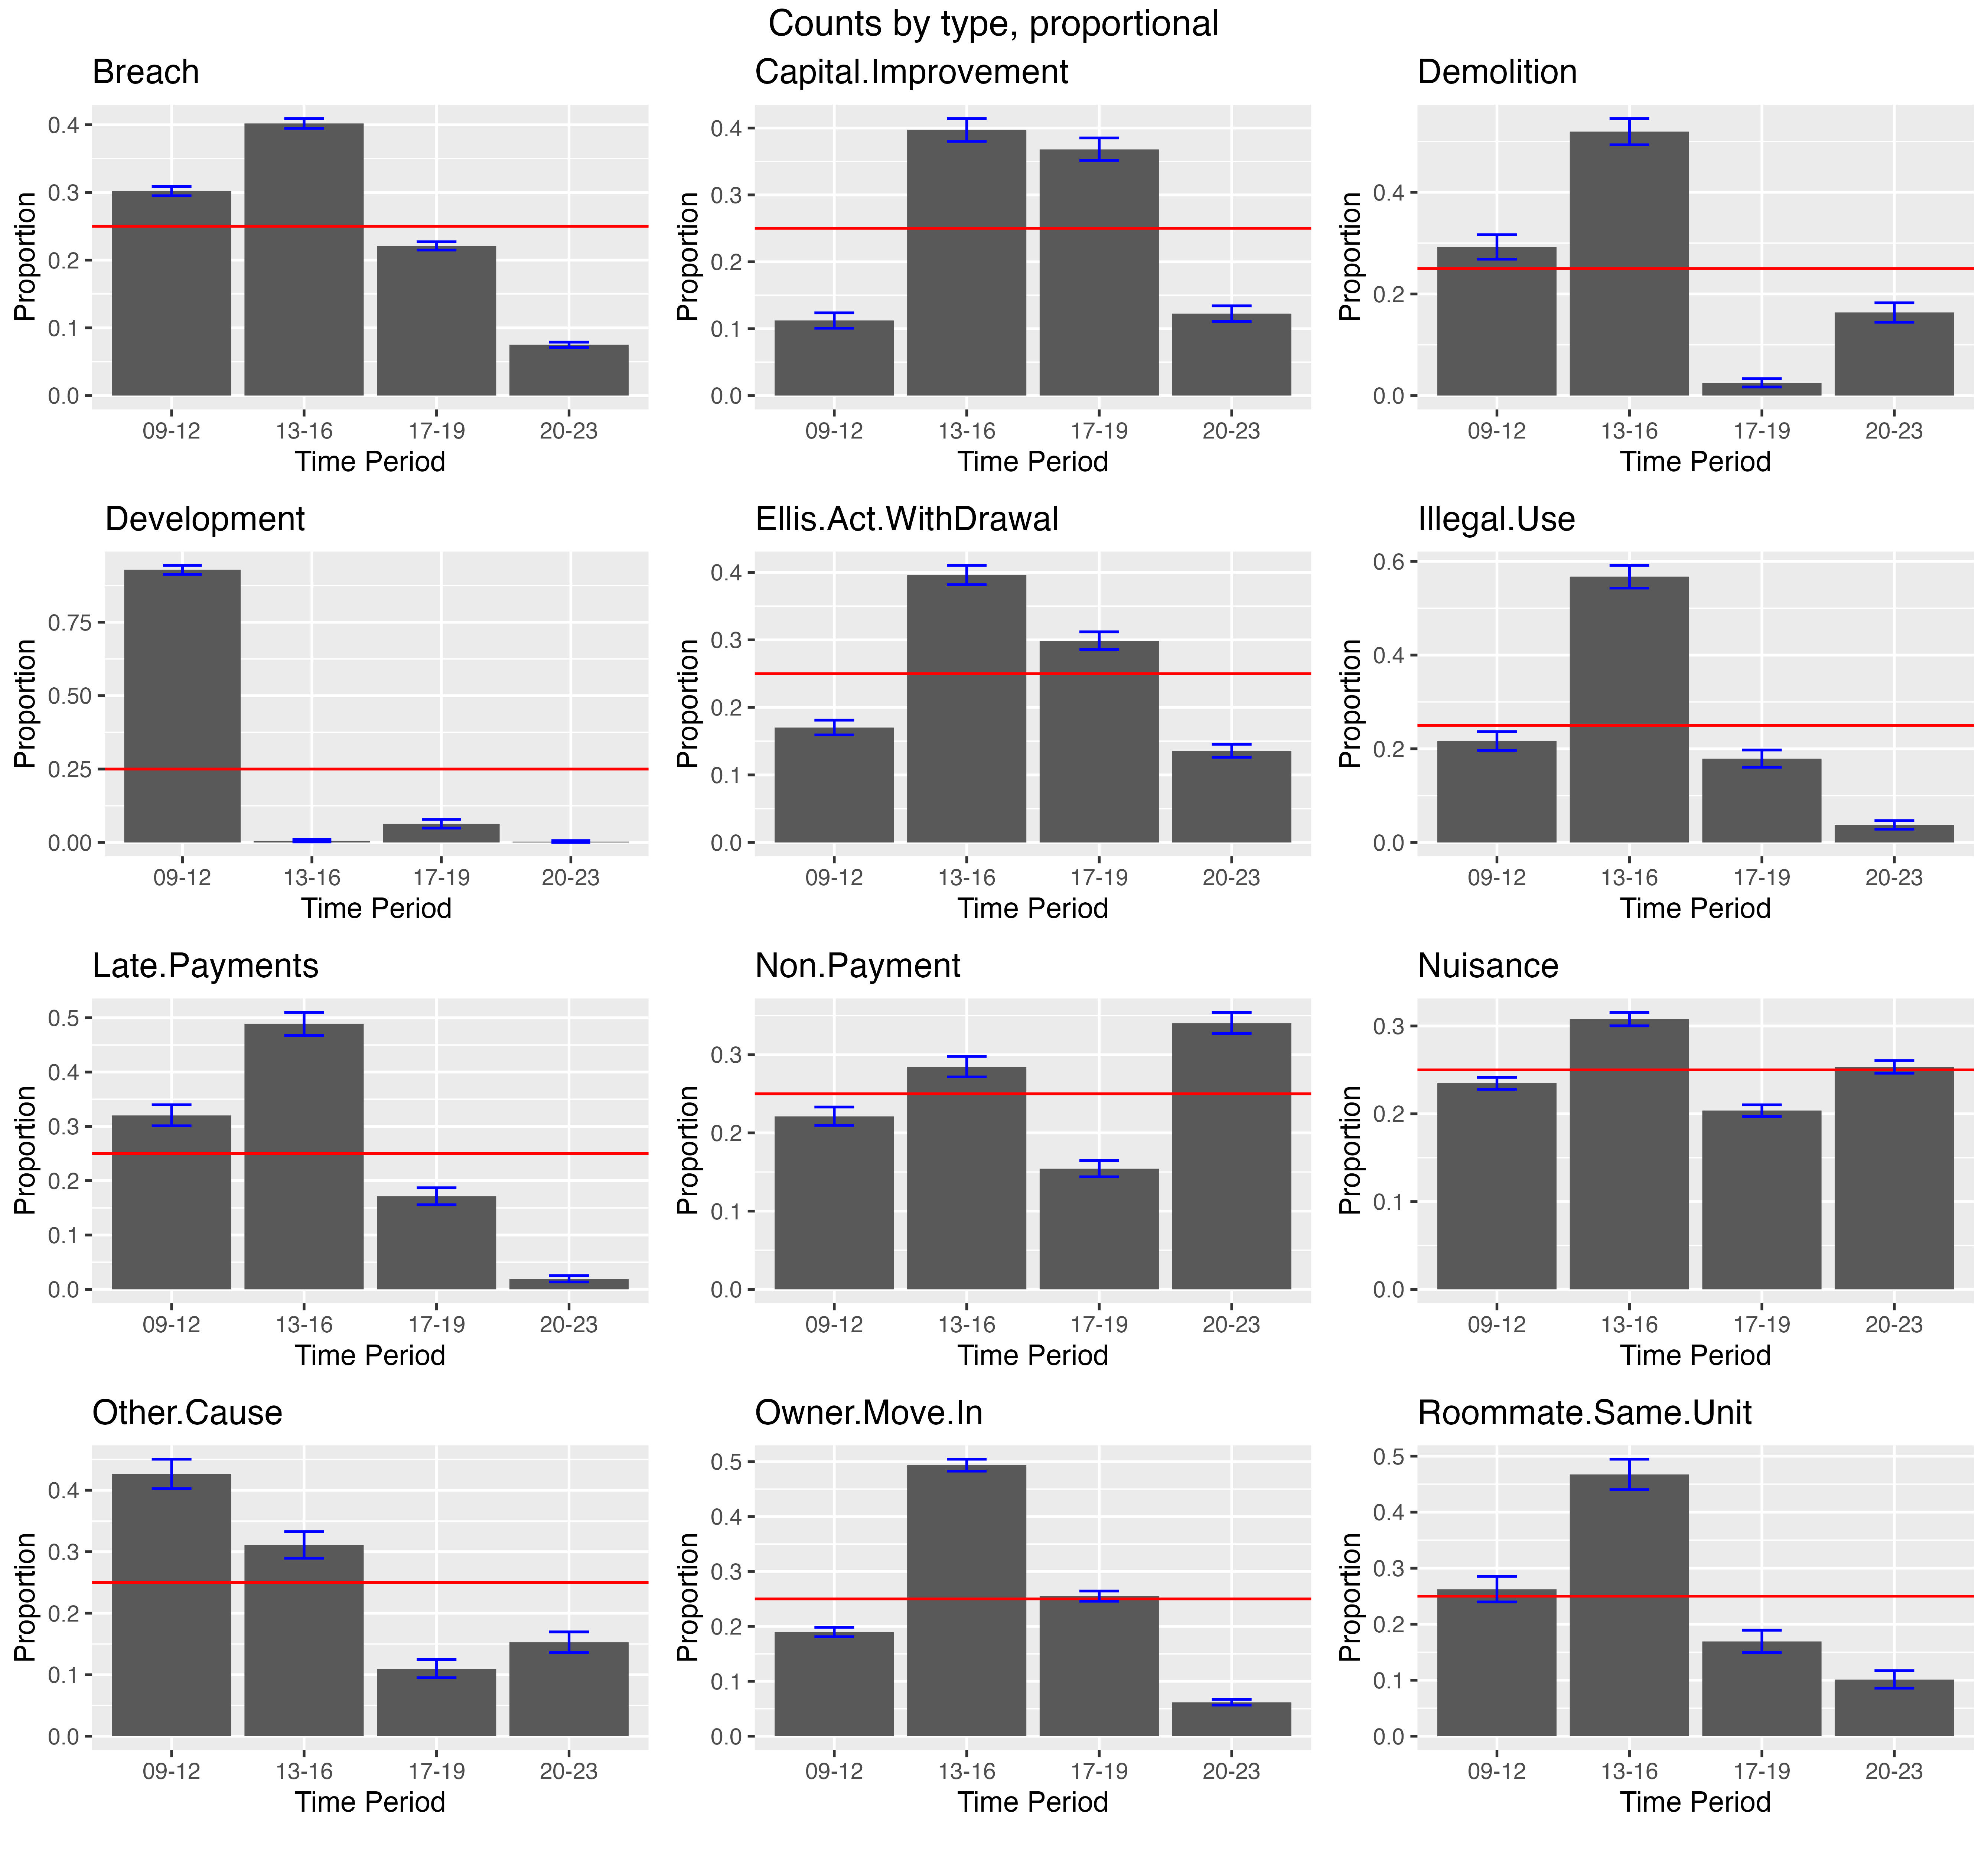
\includegraphics[width=0.8\textwidth]{/Users/brianliu03/Documents/Stats2023/data-project/test.jpg}
  \caption{Evictions by Type and Time Period (2009-23) with Expected Proportion and 99\% Confidence Intervals}
  \label{fig:test}
\end{figure}




\subsection{Calculating $z$-scores}
More importantly though, some periods have a greater deviation from the expected proportion than others. To be able to visualize and quantify this, I calculated the $z$-score for each ET in each time period.

$$
z_{t,i} = \frac{\hat{p}_{t} - p_{t,i}}{\sigma_{t,i}}
$$

where $\hat{p}_{t}$ is the expected proportion of ET $t$ and $p_{t,i}$ is the observed proportion of ET $t$ in time period $i$. $\sigma_{t,i}$ is the standard deviation of the bootstrapped samples of ET $t$ in time period $i$.

\begin{knitrout}
\definecolor{shadecolor}{rgb}{0.969, 0.969, 0.969}\color{fgcolor}\begin{kframe}
\begin{alltt}
\hlstd{signed_z_scores} \hlkwb{<-} \hlkwd{lapply}\hlstd{(}\hlnum{1}\hlopt{:}\hlnum{12}\hlstd{,} \hlkwa{function}\hlstd{(}\hlkwc{i}\hlstd{) \{}
  \hlstd{mean_prop} \hlkwb{<-} \hlkwd{get_mean_prop}\hlstd{(eviction_type[i])}
  \hlstd{ci_low} \hlkwb{<-} \hlstd{ci_bs_matrices[[i]][,} \hlnum{1}\hlstd{]}
  \hlstd{ci_high} \hlkwb{<-} \hlstd{ci_bs_matrices[[i]][,} \hlnum{2}\hlstd{]}
  \hlstd{z_scores} \hlkwb{<-} \hlkwd{numeric}\hlstd{(}\hlnum{4}\hlstd{)}
  \hlkwa{for} \hlstd{(j} \hlkwa{in} \hlnum{1}\hlopt{:}\hlnum{4}\hlstd{) \{}
    \hlkwa{if} \hlstd{(mean_prop} \hlopt{>} \hlstd{ci_high[j]) \{}
      \hlstd{z_scores[j]} \hlkwb{<-} \hlstd{(ci_high[j]} \hlopt{-} \hlstd{mean_prop)} \hlopt{/} \hlkwd{sd}\hlstd{(bs_matrices[[i]][j, ])}
    \hlstd{\}} \hlkwa{else if} \hlstd{(mean_prop} \hlopt{<} \hlstd{ci_low[j]) \{}
      \hlstd{z_scores[j]} \hlkwb{<-} \hlstd{(ci_low[j]} \hlopt{-} \hlstd{mean_prop)} \hlopt{/} \hlkwd{sd}\hlstd{(bs_matrices[[i]][j, ])}
    \hlstd{\}} \hlkwa{else} \hlstd{\{}
      \hlstd{z_scores[j]} \hlkwb{<-} \hlnum{0}
    \hlstd{\}}
  \hlstd{\}}
  \hlkwd{return}\hlstd{(z_scores)}
\hlstd{\})}
\end{alltt}
\end{kframe}
\end{knitrout}

\begin{figure}[htbp]
  \centering
  \subfigure[z-scores organized by Time Period]{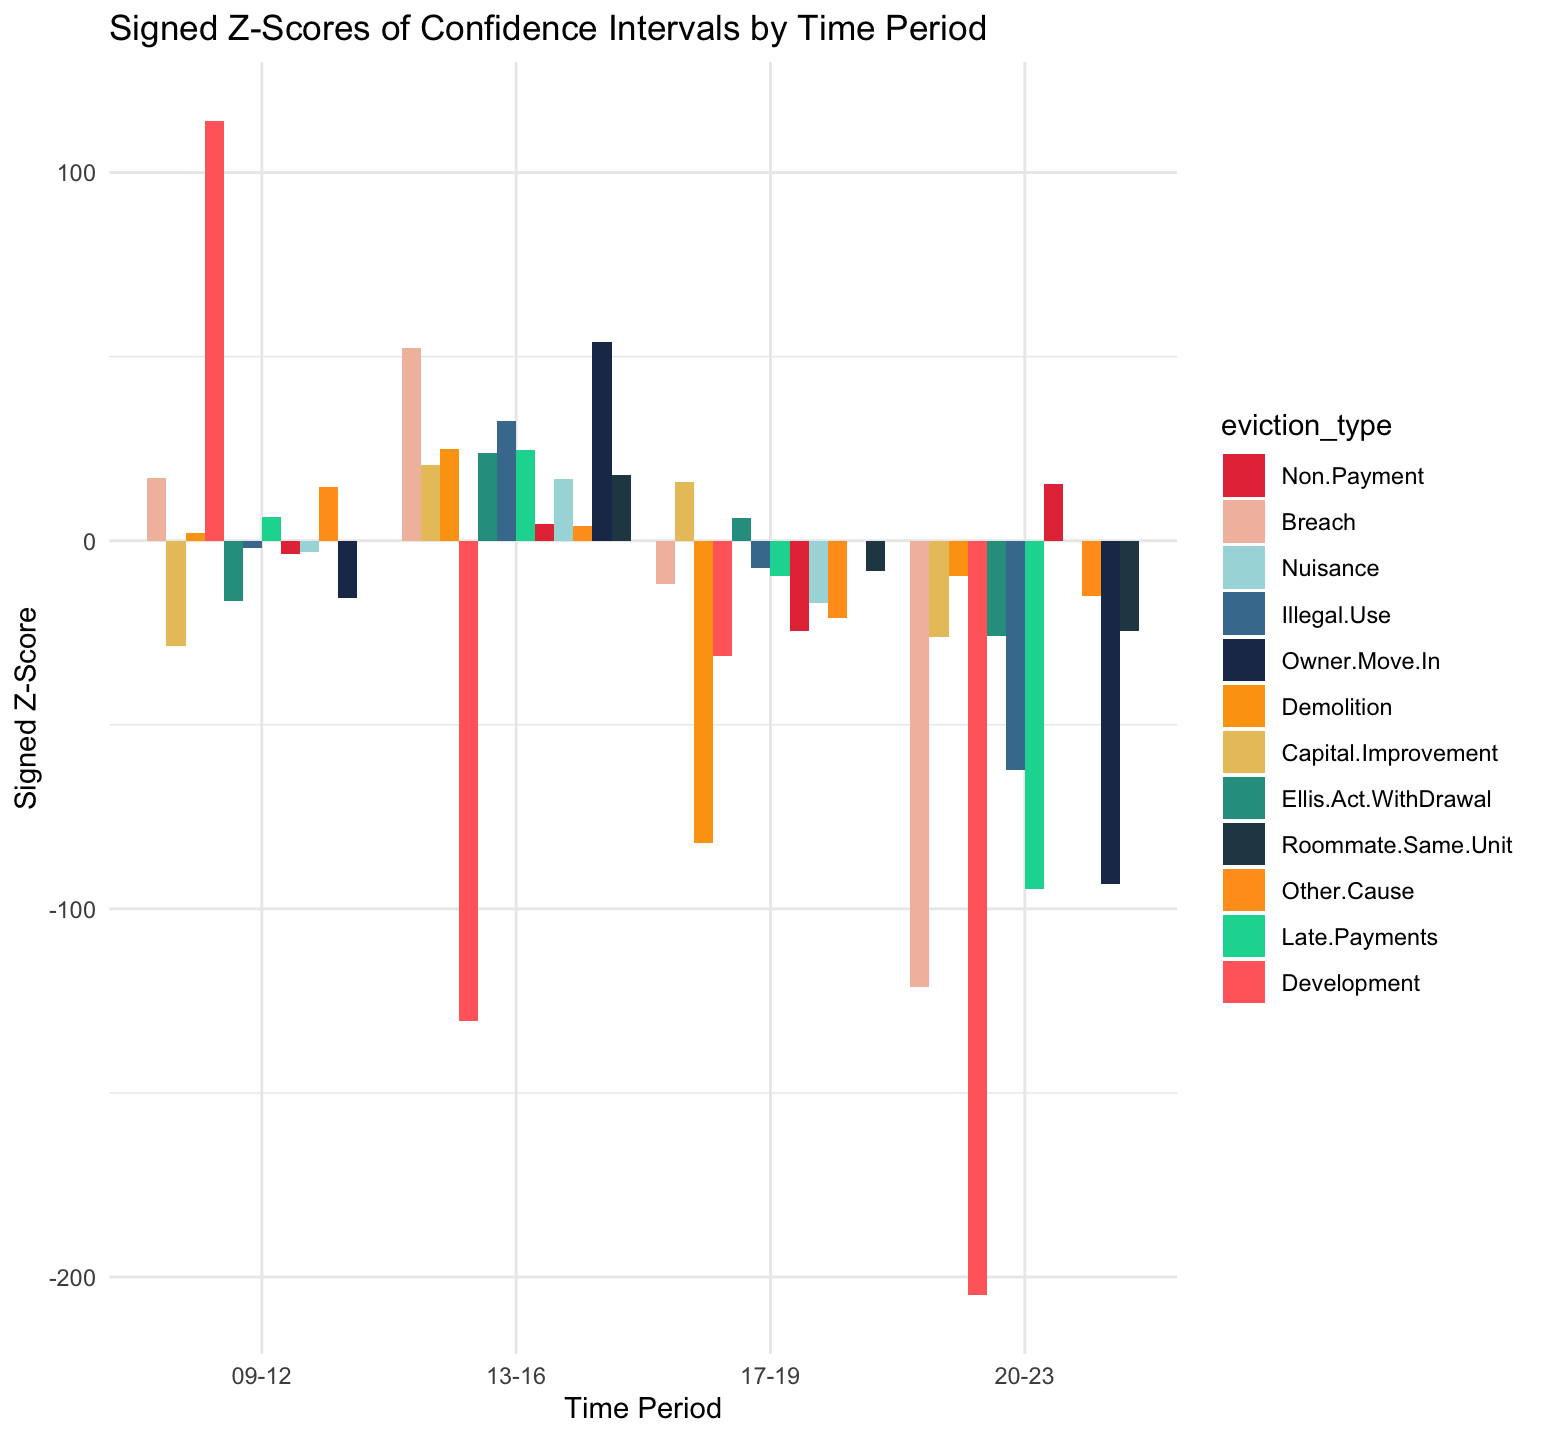
\includegraphics[width=0.7\textwidth]{/Users/brianliu03/Documents/Stats2023/data-project/images/signed_z_scores_tp.png}}
  \subfigure[z-scores organized by Time Period]{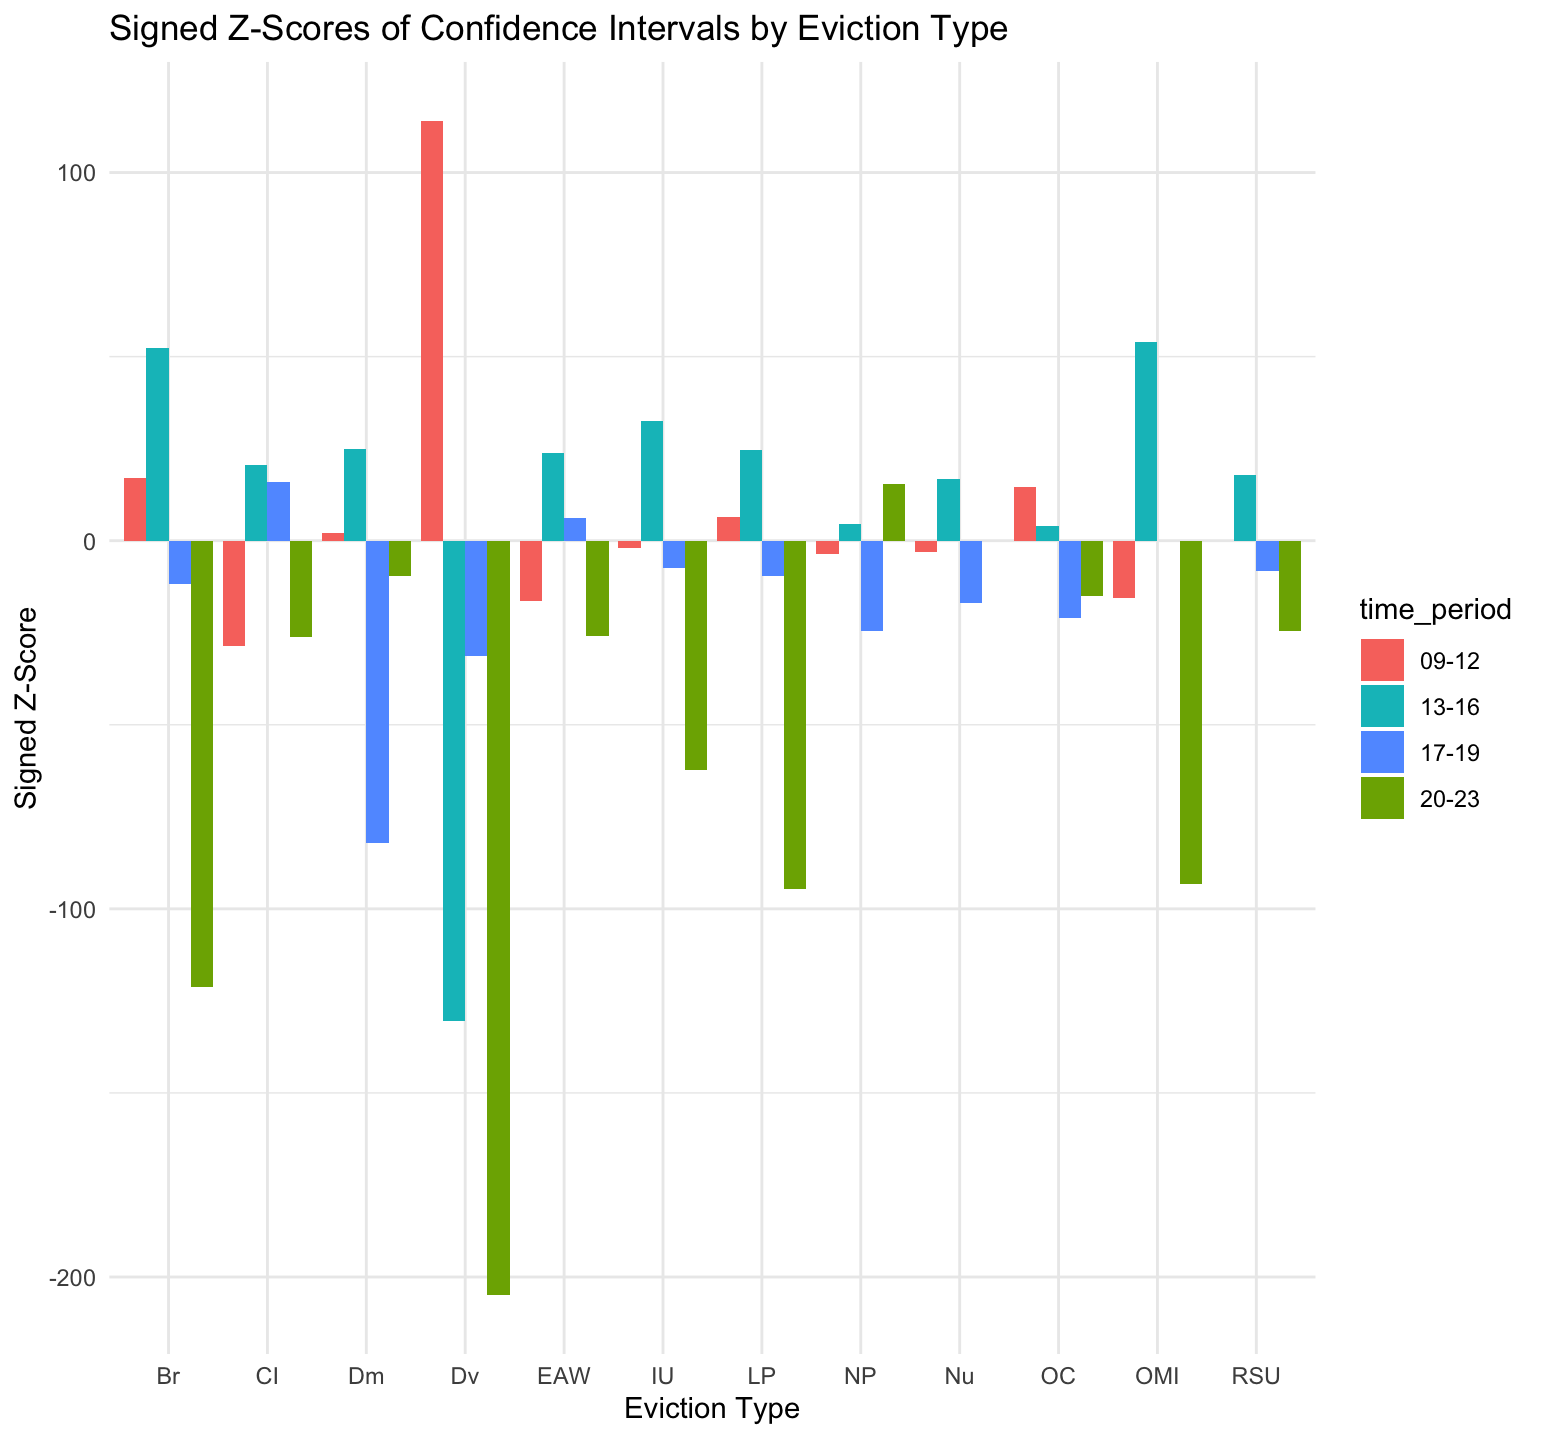
\includegraphics[width=0.7\textwidth]{/Users/brianliu03/Documents/Stats2023/data-project/images/signed_z_scores_et.png}}
  \caption{Signed z-scores by Time Period and ET}
\end{figure}

Plotting the $z$-scores allows us to see significant and varying amounts of variation for ETs and time periods. I graphed and organized them by ET and time period. These graphs allow me to perform visual hypothesis testing and find where there are significant deviations from the expected proportion. I note some observations below:

\begin{enumerate}
    \item Development evictions are significantly higher in the 2009-12 period than any other time period. There may be a correlation with the recovery from the Great Recession and the increase in development evictions.
    \item OMI evictions are significantly higher in the 2013-16 period than any other time period. This may be a result of the tech boom in the early 2010s.
    \item 2017-19 is the time period with the lesser deviation and an overall decrease in evictions. This may be a result of the local real estate market stumbling during that time.
    \item 2020-23 is the time period with the most deviation and decrease in evictions. This is most definitely a result of the pandemic.
\end{enumerate}

\section{Conclusion}
It is not like San Francisco's population has varied as significantly as the eviction rates have. From this data we can see that eviction comes in waves, whether that be from seasons, the real estate market, a pandemic, a tech boom, or any other factor that affects the balance of capitalism. With each of these events comes different strategies landlords use to evict tenants.

My exploration of the subsetted data from 2009-23 shows that there is a lot of variation in evictions types and filing patterns, and it is important to understand the context of the time period to understand the eviction rates. The map plots also show that there are certain neighborhoods that are more affected by evictions than others, and these neighborhoods are the ones that have been historically redlined.

\subsection{Limitations and Future Work}
The housing crisis is an incredibly complex topic, and it would be a disservice to not go over at least some of the limitations of this paper. This data set does not include eviction notices from single-room occupancies (SROs), which naturally have a lot of movement in housing and evictions. If one examines the evictions in here closely, the reasons for evictions and intentions are completely different. A lot of people coming to SROs have dealt with trauma from homelessness or other events, and they usually are not getting the support they need. In fact, coming into SROs often entail conforming to strict regulations including zero-tolerance for visitors and curfews.

Evictions are also not the only way people are displaced from their homes. There are other ways that people are displaced from their homes, such as buyouts, harassment, and other strategies that landlords use to get tenants to leave. This data set does not include these other strategies, and it would be interesting to see how these strategies have changed over time.

Finally, I have not fully explored this data set. There is a lot more to explore with the spatial aspect of this data set, and I would like to explore the spatial patterns of evictions in San Francisco. I would also like to explore the relationship between evictions and other variables such as housing prices, rents, and demographics.

% now make bibliography
% use these bibs
% Eviction Notices in SF Data Set: DataSF and SF Rent Board. Retrieved from \textit{https://data.sfgov.org/Housing-and-Buildings/Eviction-Notices/5cei-gny5}
    
% Capps, K. (2014). Peak Eviction Came to San Francisco Back in the 1990s. \textit{Bloomberg}. Retrieved from \textit{https://www.bloomberg.com/news/articles/2014-06-04/peak-eviction-came-to-san-francisco-back-in-the-1990s}

% Central Market/Tenderloin Poverty Portal. Retrieved from \textit{https://cmtldata.org/data/poverty}

% Brinklow, A. (n.d.). Eviction notices in San Francisco down for the first time since 2010. Retrieved from \textit{https://cdn2.hubspot.net/hubfs/4408380/PDF/Eviction-Reports-Articles-Cities-States/eviction-sf-decline-tec.pdf}

% Tracy, J. (n.d.). A Decade of Displacement. \textit{FoundSF}. Retrieved from \url{https://www.foundsf.org/index.php?title=A_Decade_of_Displacement}

\section*{References}

\begin{enumerate}
  \item Eviction Notices in SF Data Set: DataSF and SF Rent Board. Retrieved from \textit{https://data.sfgov.org/Housing-and-Buildings/Eviction-Notices/5cei-gny5}
  \item Capps, K. (2014). Peak Eviction Came to San Francisco Back in the 1990s. \textit{Bloomberg}. Retrieved from \textit{https://www.bloomberg.com/news/articles/2014-06-04/peak-eviction-came-to-san-francisco-back-in-the-1990s}
  \item Central Market/Tenderloin Poverty Portal. Retrieved from \textit{https://cmtldata.org/data/poverty}
  \item Brinklow, Eviction notices in San Francisco down for the first time since 2010. Retrieved from \\ \textit{https://cdn2.hubspot.net/hubfs/4408380/PDF/Eviction-Reports-Articles-Cities-States/eviction-sf-decline-tec.pdf}
  \item Tracy, A Decade of Displacement. Retrieved from \textit{https://www.foundsf.org/index.php?title=A\_Decade\_of\_Displacement}
\end{enumerate}

\end{document}
